\chapter*{Introduction}


\begin{figure}
\centering
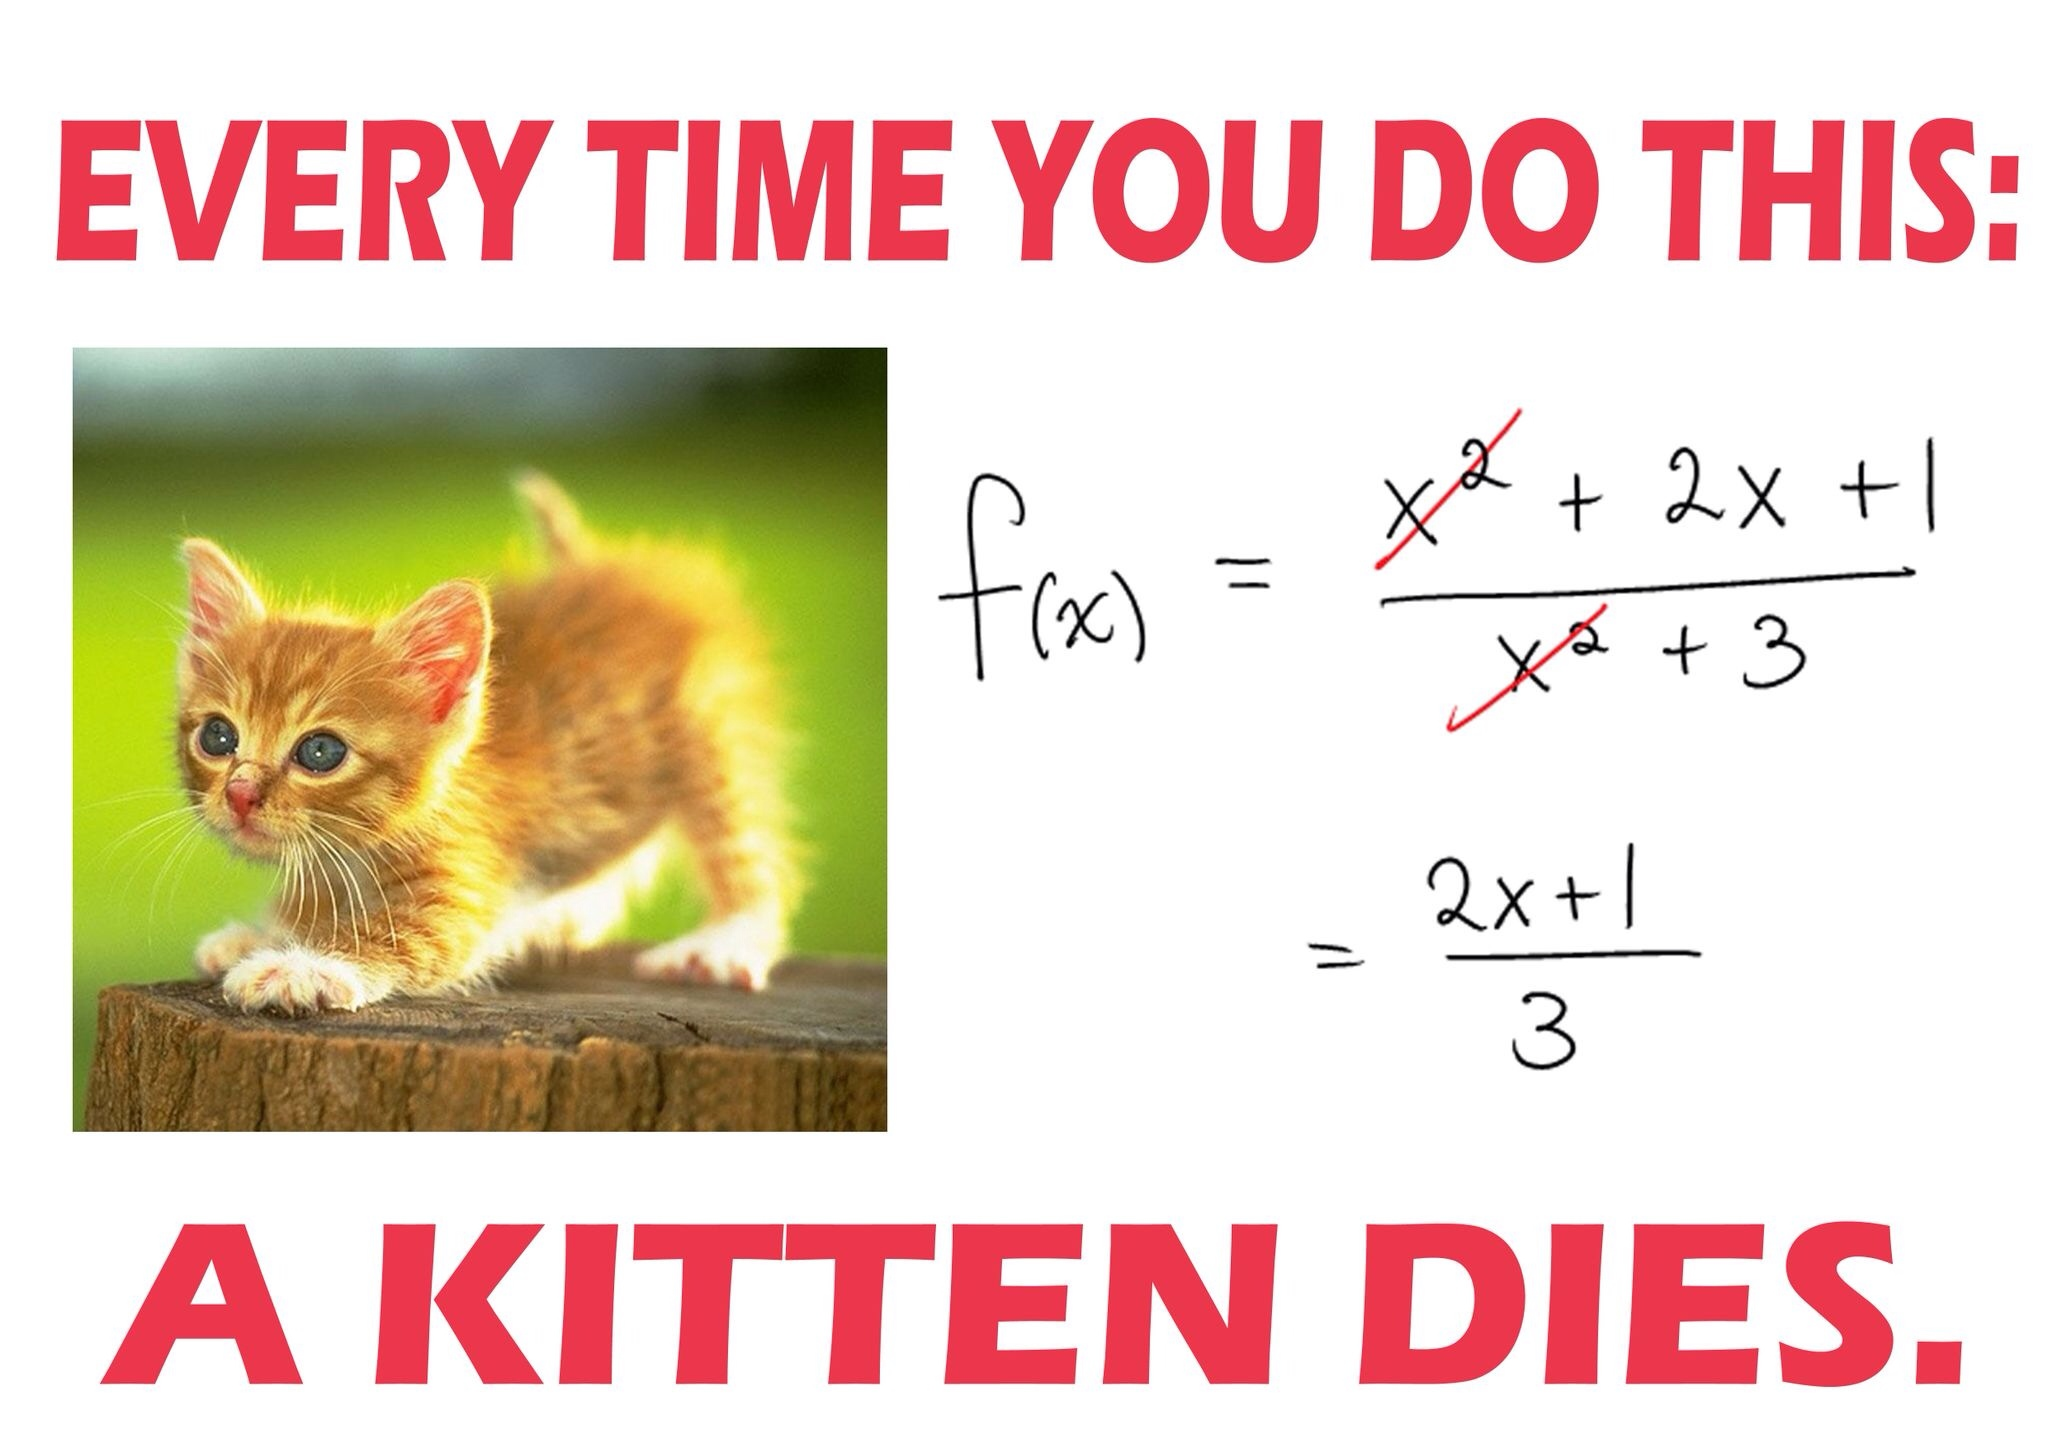
\includegraphics[width=6cm]{picture/obr.jpg}
\caption{A completed nonogram}
\end{figure}

\textbf{Nonograms}, also known as \textbf{Hanjie}, \textbf{Picross} or \textbf{Griddlers}, are picture \textit{logic puzzles} in which cells in a grid must be colored or left blank according to numbers at the side of the grid to reveal a hidden picture. In this puzzle type, the numbers are a form of \textit{discrete tomography} that measures how many unbroken lines of filled-in squares there are in any given row or column. For example, a clue of "4 8 3" would mean there are sets of four, eight, and three filled squares, in that order, with at least one blank square between successive groups.

These puzzles are often black and white, describing a \textit{binary image}, but they can also be colored. If colored, the number clues are also colored to indicate the color of the squares. Two differently colored numbers may or may not have a space in between them. For example, a black four followed by a red two could mean four black boxes, some empty spaces, and two red boxes, or it could simply mean four black boxes followed immediately by two red ones.

Nonograms have no theoretical limits on size, and are not restricted to square layouts.


\chapter{Names}

Nonograms are also known by many other names, including Paint by Numbers, Griddlers, Pic-a-Pix, Picross, PrismaPixels, Pixel Puzzles, Crucipixel, Edel, FigurePic, Hanjie, HeroGlyphix, Illust-Logic, Japanese \textit{Crosswords}, Japanese Puzzles, Kare Karala!, Logic Art, Logic Square, Logicolor, Logik-Puzzles, Logimage, Oekaki Logic, Oekaki-Mate, Paint Logic, Picture Logic, Tsunamii, Paint by \textit{Sudoku} and \textit{Binary} Coloring Books.


\chapter{History}
In 1987, Non Ishida, a Japanese graphics editor, won a competition in Tokyo by designing grid pictures using skyscraper lights that were turned on or off. Coincidentally, a professional Japanese puzzler named Tetsuya Nishio invented the same puzzles.(TODO - referencia na literaturu)


\section{Print publishing}
Paint by numbers puzzles started appearing in Japanese puzzle magazines. Non Ishida published three picture grid puzzles in 1988 in Japan under the name of "Window Art Puzzles". Subsequently in 1990, James Dalgety in the UK invented the name Nonograms after Non Ishida, and \textit{\textit{The Sunday Telegraph}} started publishing them on a weekly basis. By 1993, First book of Nonograms was published by Non Ishida in Japan. The \textit{Sunday Telegraph} published a dedicated puzzle book titled the "Book of Nonograms". Nonograms were also published in Sweden, United States (originally by \textit{\textit{Games} magazine}(TODO - referencia na literaturu)), South Africa and other countries. The \textit{Sunday Telegraph} ran a competition in 1998 to choose a new name for their puzzles. Griddlers was the winning name that readers chose.


\section{Electronic puzzles}
Paint by numbers puzzles were implemented by 1995 on hand held electronic toys such as Game Boy and on other plastic puzzle toys. \textit{Nintendo} picked up on this puzzle \textit{fad} and released two "Picross" (\textbf{Pic}ture \textbf{Cross}word) titles for the \textit{Game Boy} and nine for the \textit{Super Famicom} (eight of which were released in two-month intervals for the Nintendo Power Super Famicom Cartridge Writer as the "NP Picross" series) in Japan. Only one of these, \textit{\textit{Mario's Picross}} for the Game Boy, was released outside Japan. Another version, \textit{Picross DS} was released in 2007. Another downloadable series of Picross was also released for Nintendo 3DS's Nintendo eShop, called \textit{Picross e} currently consists of 7 "Picross e" titles.  Increased popularity in Japan launched new publishers and by now there were several monthly magazines, some of which contained up to 100 puzzles. The Japanese arcade game Logic Pro was released by Deniam Corp in 1996, with a sequel released the following year. UK games developer Jagex released a nonogram puzzle in 2011 as part of their annual Halloween event for their java based game, Runescape. In 2013, Casual Labs released a mobile version of these puzzles called "Paint it Back" with the theme of restoring an art gallery.


\section{Today}
Paint by numbers have been published by Sanoma Uitgevers in the Netherlands, Puzzler Media (formerly British European Associated Publishers) in the UK and Nikui Rosh Puzzles in Israel. Magazines with nonogram puzzles are published in the USA, UK, Germany, Netherlands, Italy, Hungary, Finland, Ukraine, and many other countries.


\chapter{Solution techniques}

\begin{figure}
\centering
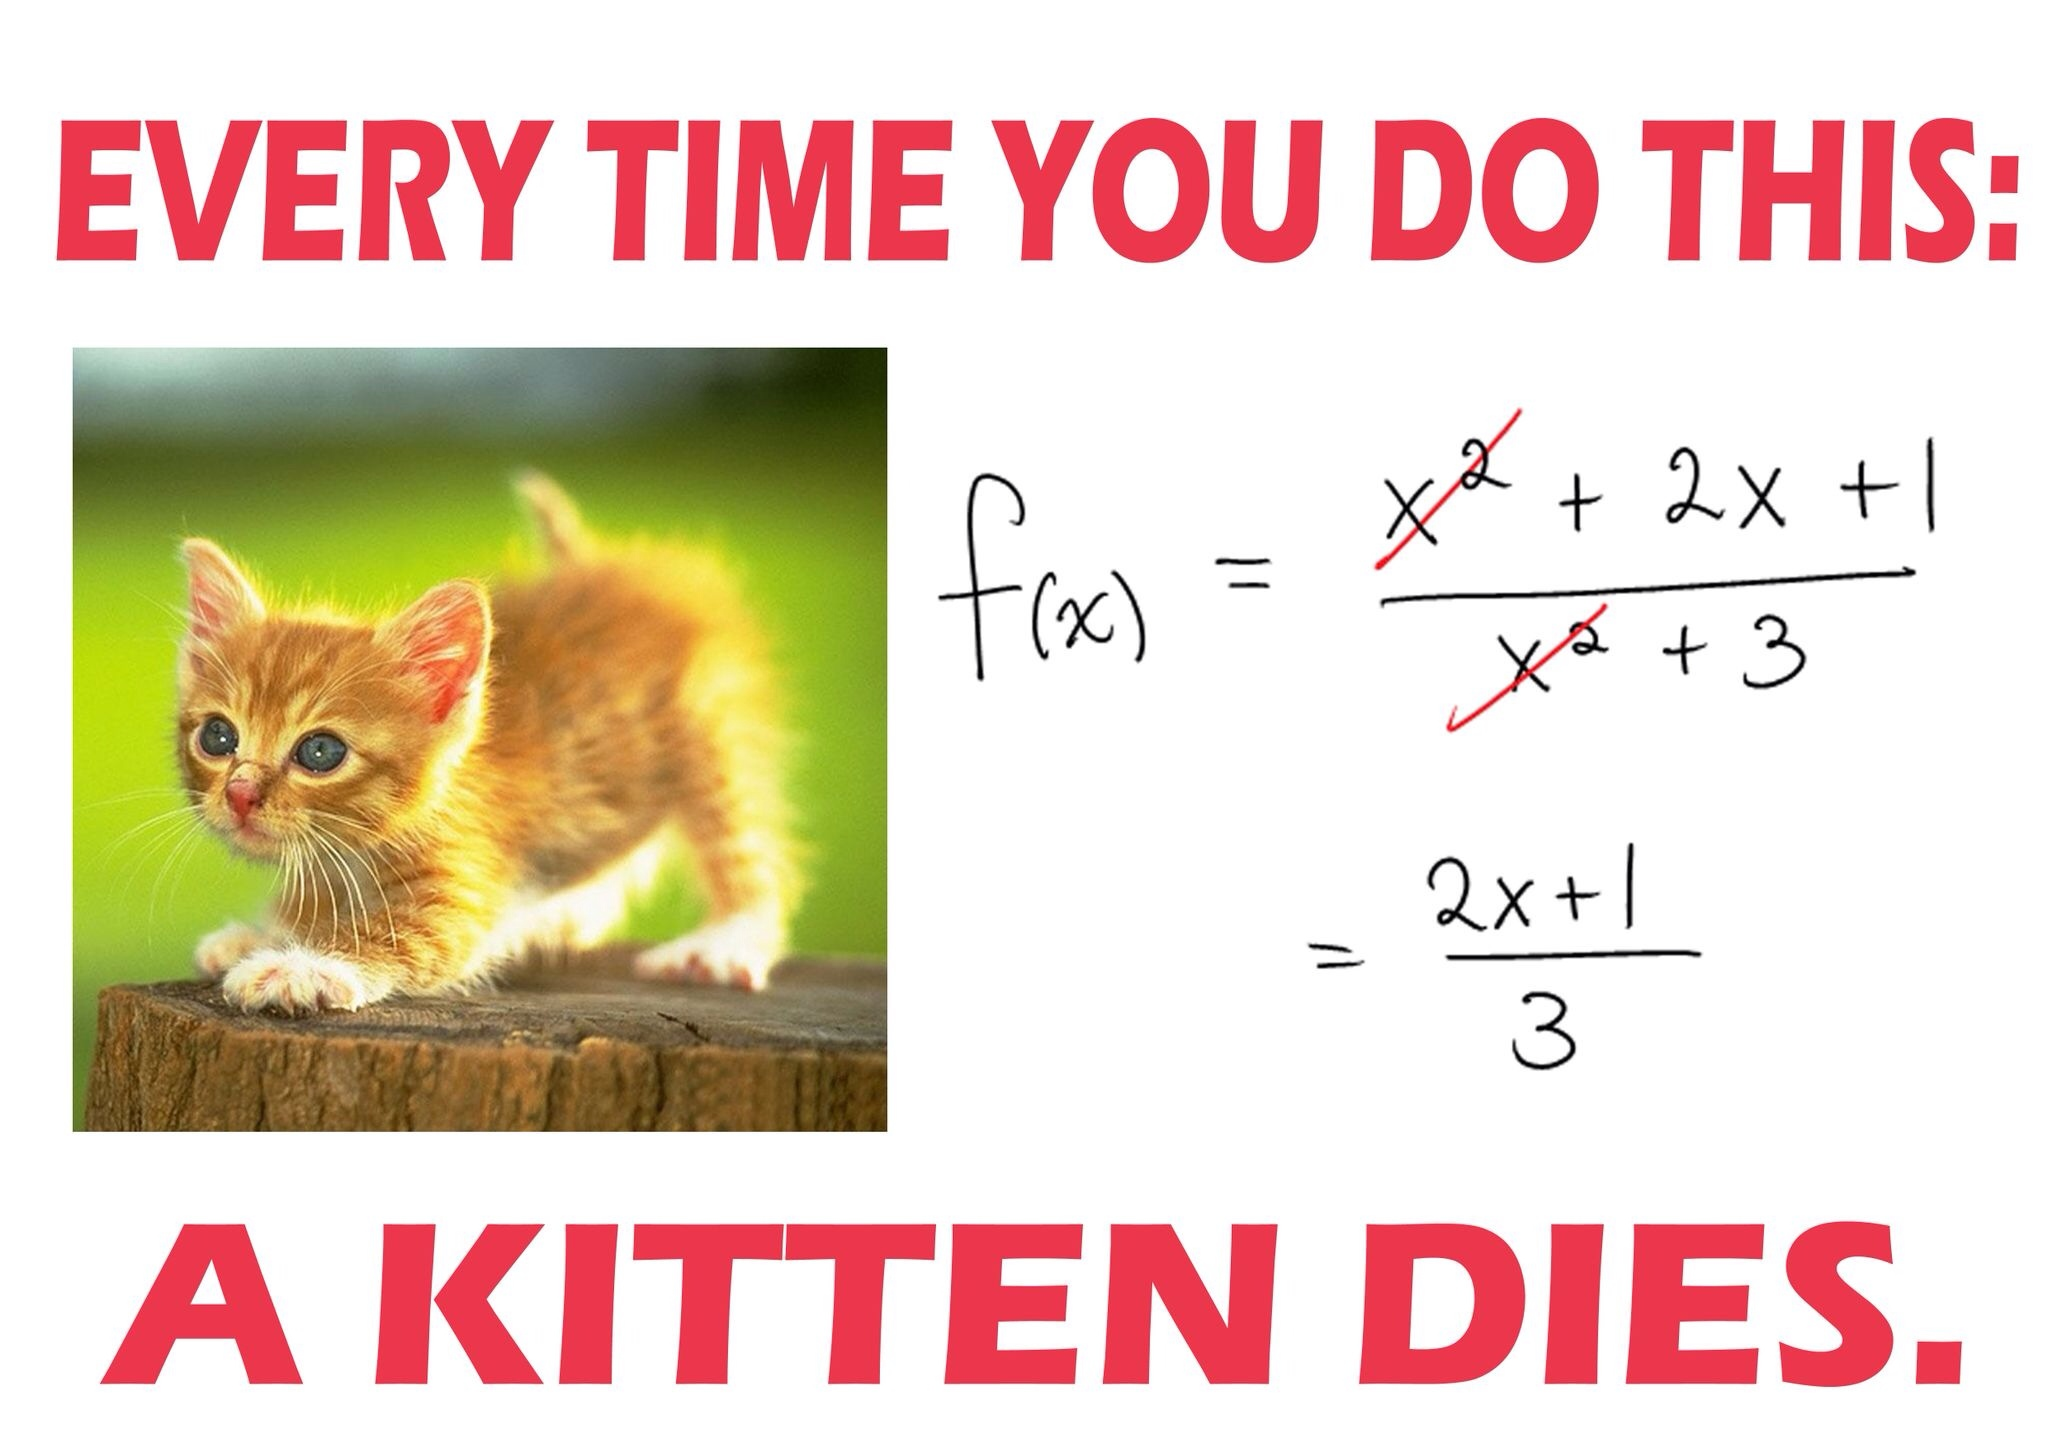
\includegraphics[width=6cm]{picture/obr.jpg}
\caption{Example of a nonogram puzzle being solved. Some of the steps of the process are grouped together.}
\end{figure}

To solve a puzzle, one needs to determine which cells will be boxes and which will be empty. Determining which cells are to be left empty (called spaces) is as important as determining which to fill (called boxes). Later in the solving process, the spaces help determine where a clue (continuing block of boxes and a number in the legend) may spread. Solvers usually use a dot or a cross to mark cells they are certain are spaces.

It is also important never to guess. Only cells that can be determined by logic should be filled. If guessing, a single error can spread over the entire field and completely ruin the solution. It usually comes to the surface only after a while, when it is very difficult to correct the puzzle. Usually, only advanced and experienced solvers are able to fix it completely and finish such ruined puzzles.

The hidden picture plays no part in the solving process. Even if it is obvious from the picture that a cell will be a box, it is usually treacherous to rely on it. The picture, however, may help find and eliminate an error.

Simpler puzzles can usually be solved by a reasoning on a single row only (or a single column) at each given time, to determine as many boxes and spaces on that row as possible. Then trying another row (or column), until there are no rows that contain undetermined cells.

Some more difficult puzzles may also require several types of "what if?" reasoning that include more than one row (or column). This works on searching for contradictions: \textit{When a cell cannot be a box, because some other cell would produce an error, it will definitely be a space. And vice versa.} Advanced solvers are sometimes able to search even deeper than into the first "what if?" reasoning. It takes, however, a lot of time to get some progress.


\section{Simple boxes}
At the beginning of the solution a simple method can be used to determine as many boxes as possible. This method uses conjunctions of possible places for each block of boxes. For example, in a row of ten cells with only one clue of \textit{8}, the bound block consisting of 8 boxes could spread from
\begin{figure}
\centering
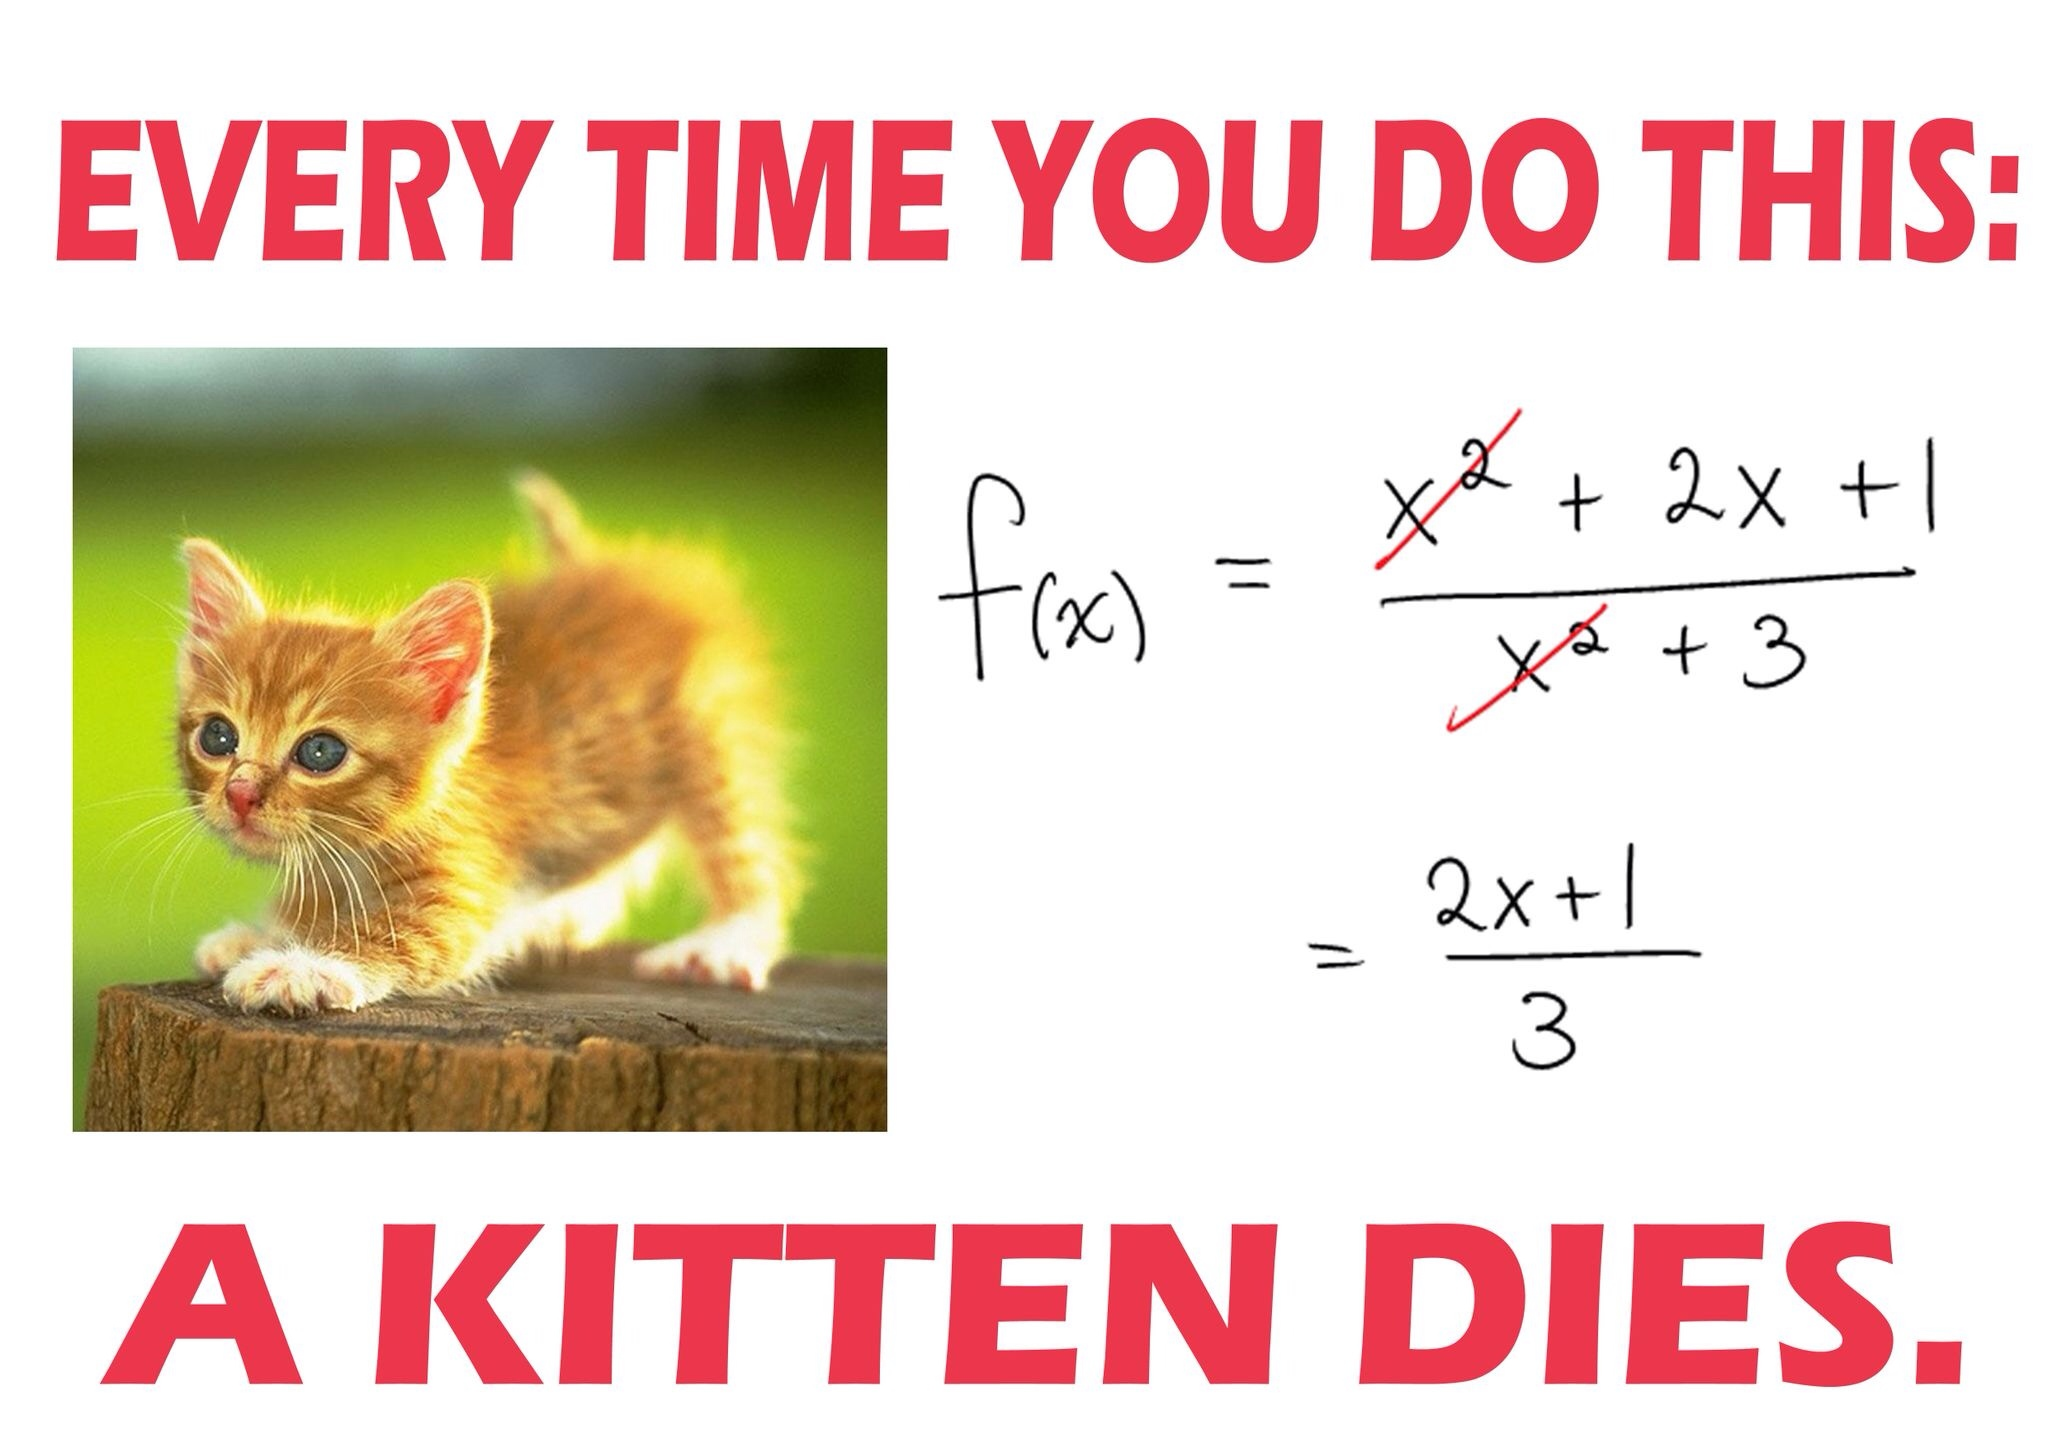
\includegraphics[width=6cm]{picture/obr.jpg}
\end{figure}

\begin{itemize} 
 \item {the right border, leaving two spaces to the left;}

\item {the left border, leaving two spaces to the right;}

\item {or somewhere in between.} 
\end{itemize}

As a result, the block \textbf{must} spread through the six centermost cells in the row.

The same of course applies when there are more clues in the row. For example, in a row of ten cells with clues of \textit{4} and \textit{3}, the bound blocks of boxes could be
\begin{figure}
\centering
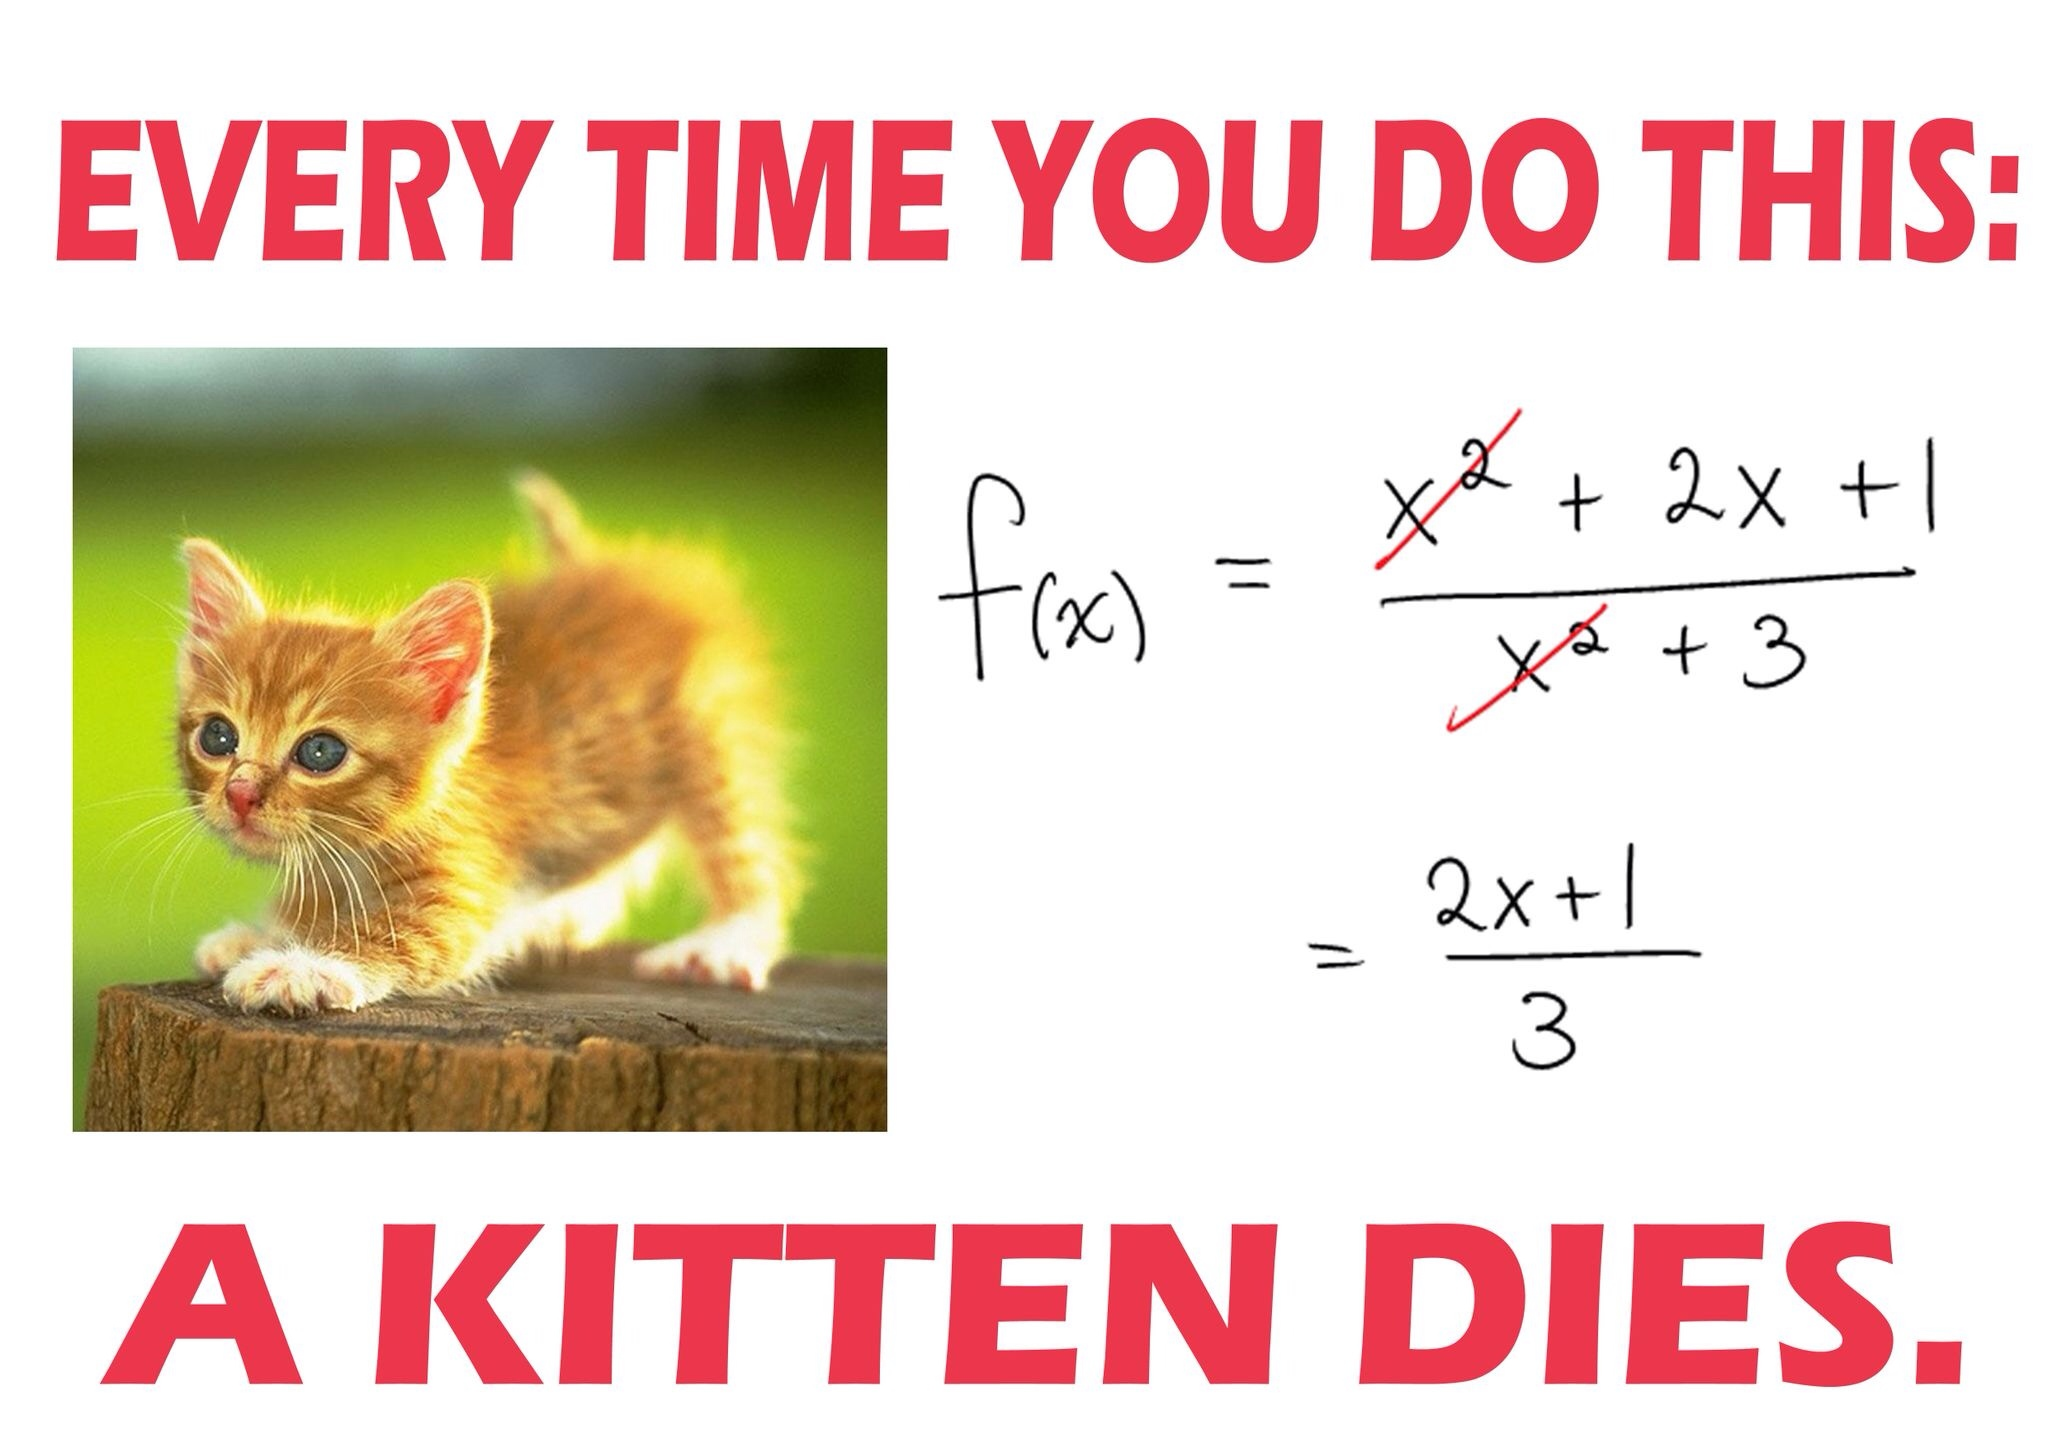
\includegraphics[width=6cm]{picture/obr.jpg}
\end{figure}

\begin{itemize} 
 \item {crowded to the left, one next to the other, leaving two spaces to the right;}

\item {crowded to the right, one just next to the other, leaving two spaces to the left;}

\item {or somewhere between.} 
\end{itemize}

Consequently, the first block of four boxes definitely includes the third and fourth cells, while the second block of three boxes definitely includes the eighth cell. Boxes can therefore be placed in the third, fourth and eighth cells. Important note: When determining boxes in this way, boxes can be placed in cells only when the same block overlaps; in this example, although two blocks overlap in the sixth cell, they are different blocks, and so it cannot yet be said whether or not the sixth cell will contain a box.


\section{Simple spaces}
This method consists of determining spaces by searching for cells that are out of range of any possible blocks of boxes. For example, considering a row of ten cells with boxes in the fourth and ninth cell and with clues of \textit{3} and \textit{1}, the block bound to the clue \textit{3} will spread through the fourth cell and clue \textit{1} will be at the ninth cell.
\begin{figure}
\centering
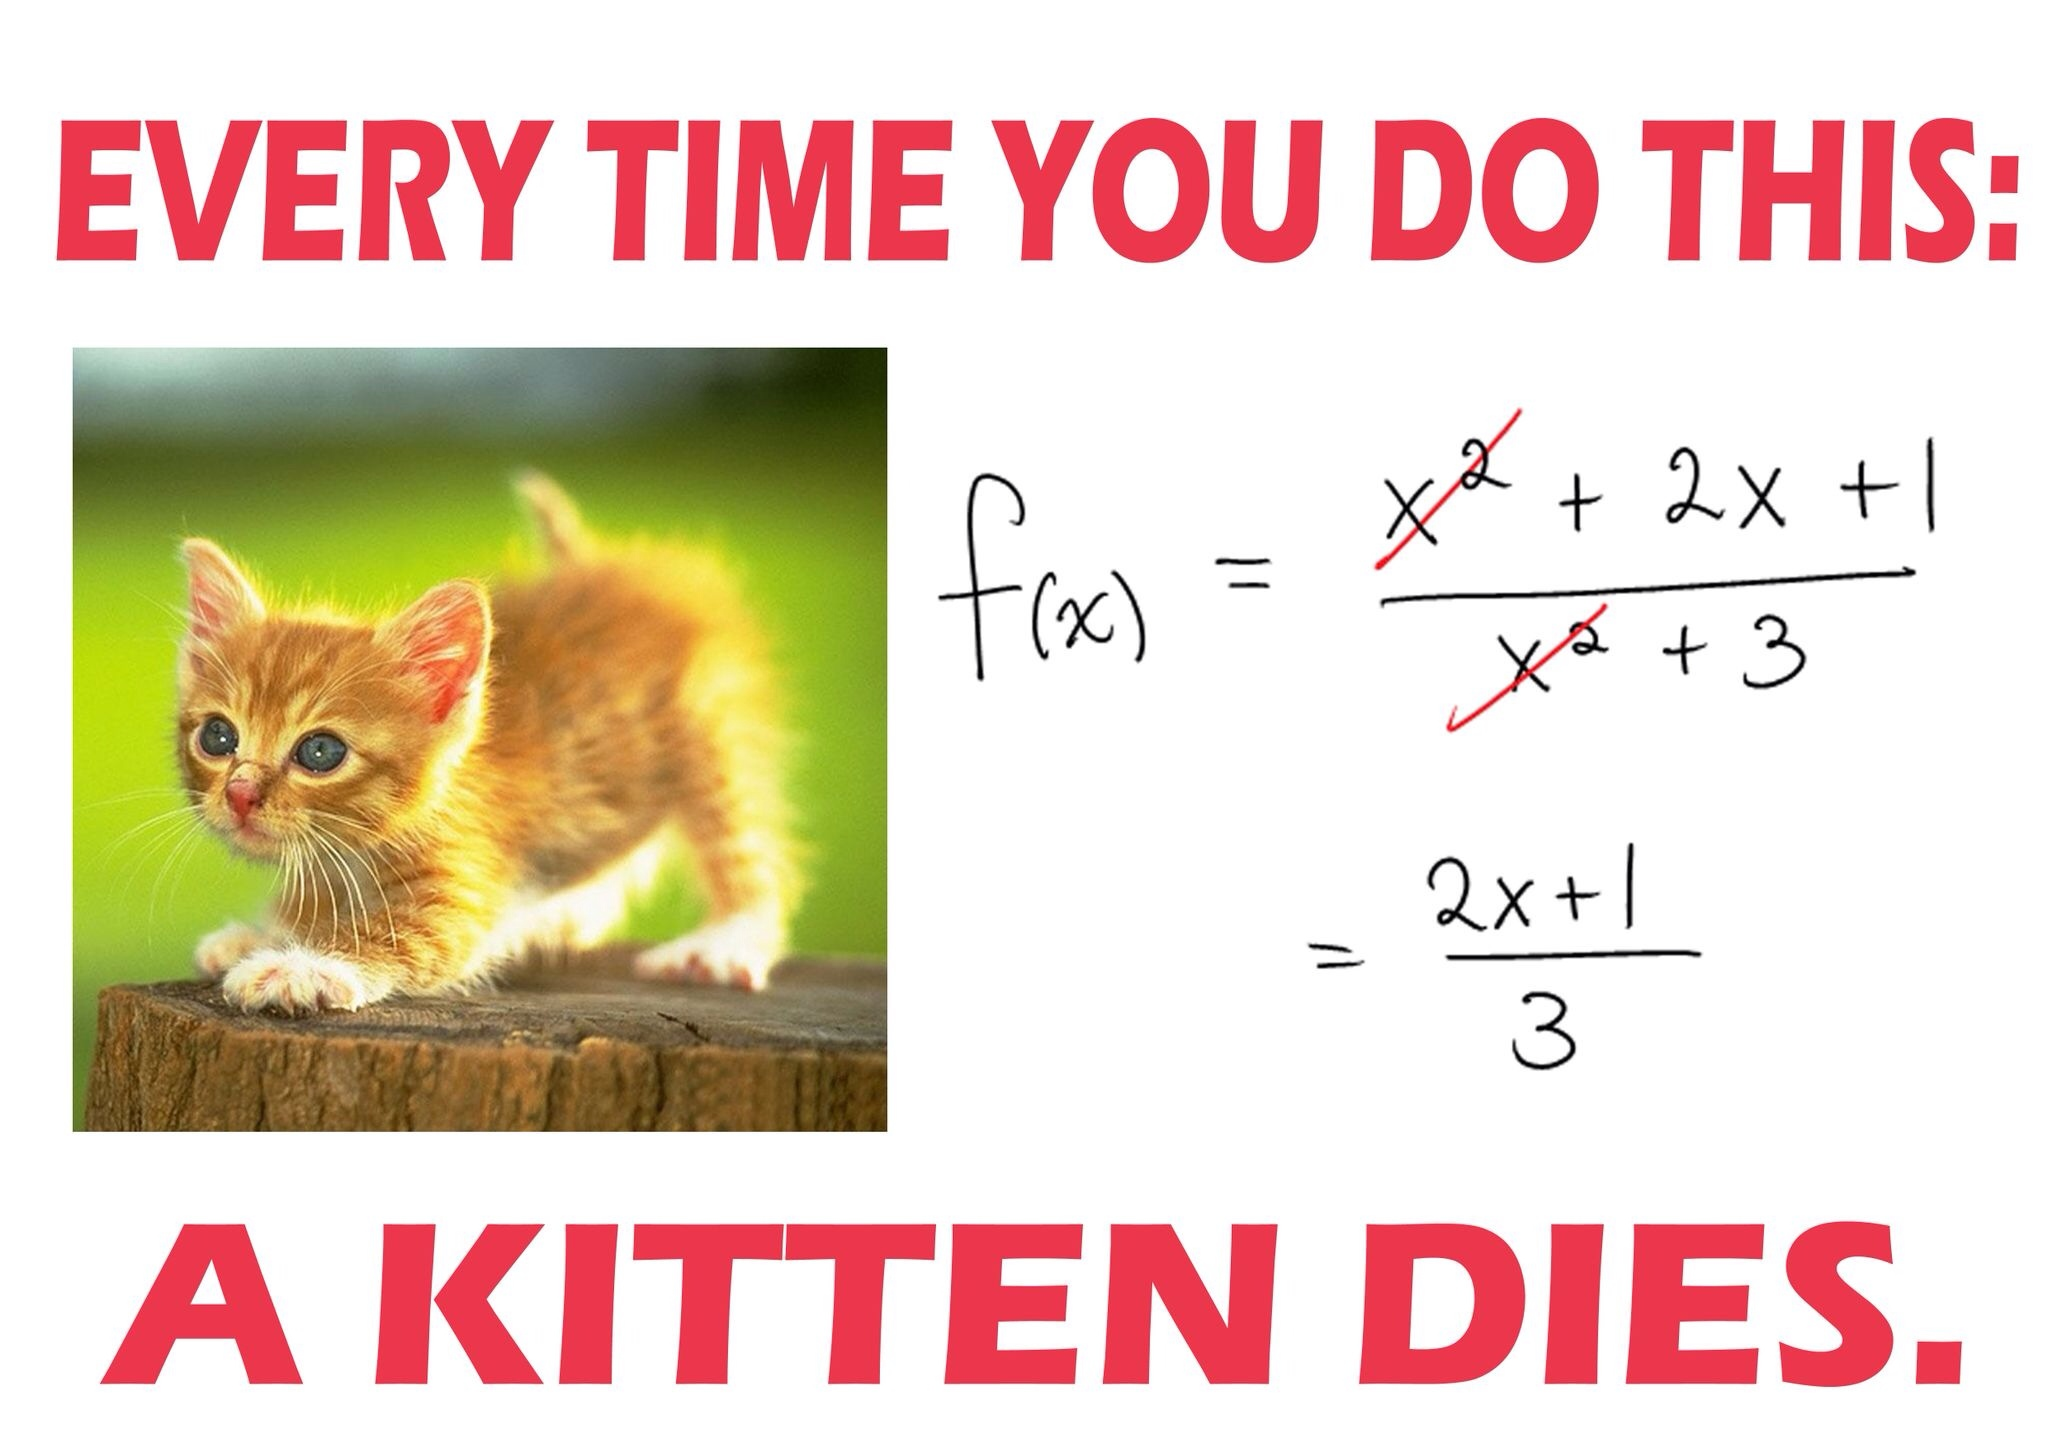
\includegraphics[width=6cm]{picture/obr.jpg}
\end{figure}
First, the clue \textit{1} is complete and there will be a space at each side of the bound block.

Second, the clue \textit{3} can only spread somewhere between the second cell and the sixth cell, because it always has to include the fourth cell; however, this may leave cells that may not be boxes in any case, i.e. the first and the seventh.

Note: In this example all blocks are accounted for; this is not always the case. The player must be careful for there may be clues or blocks that are not bound to each other yet.


\section{Forcing}
In this method, the significance of the spaces will be shown. A space placed somewhere in the middle of an uncompleted row may force a large block to one side or the other. Also, a gap that is too small for any possible block may be filled with spaces.
\begin{figure}
\centering
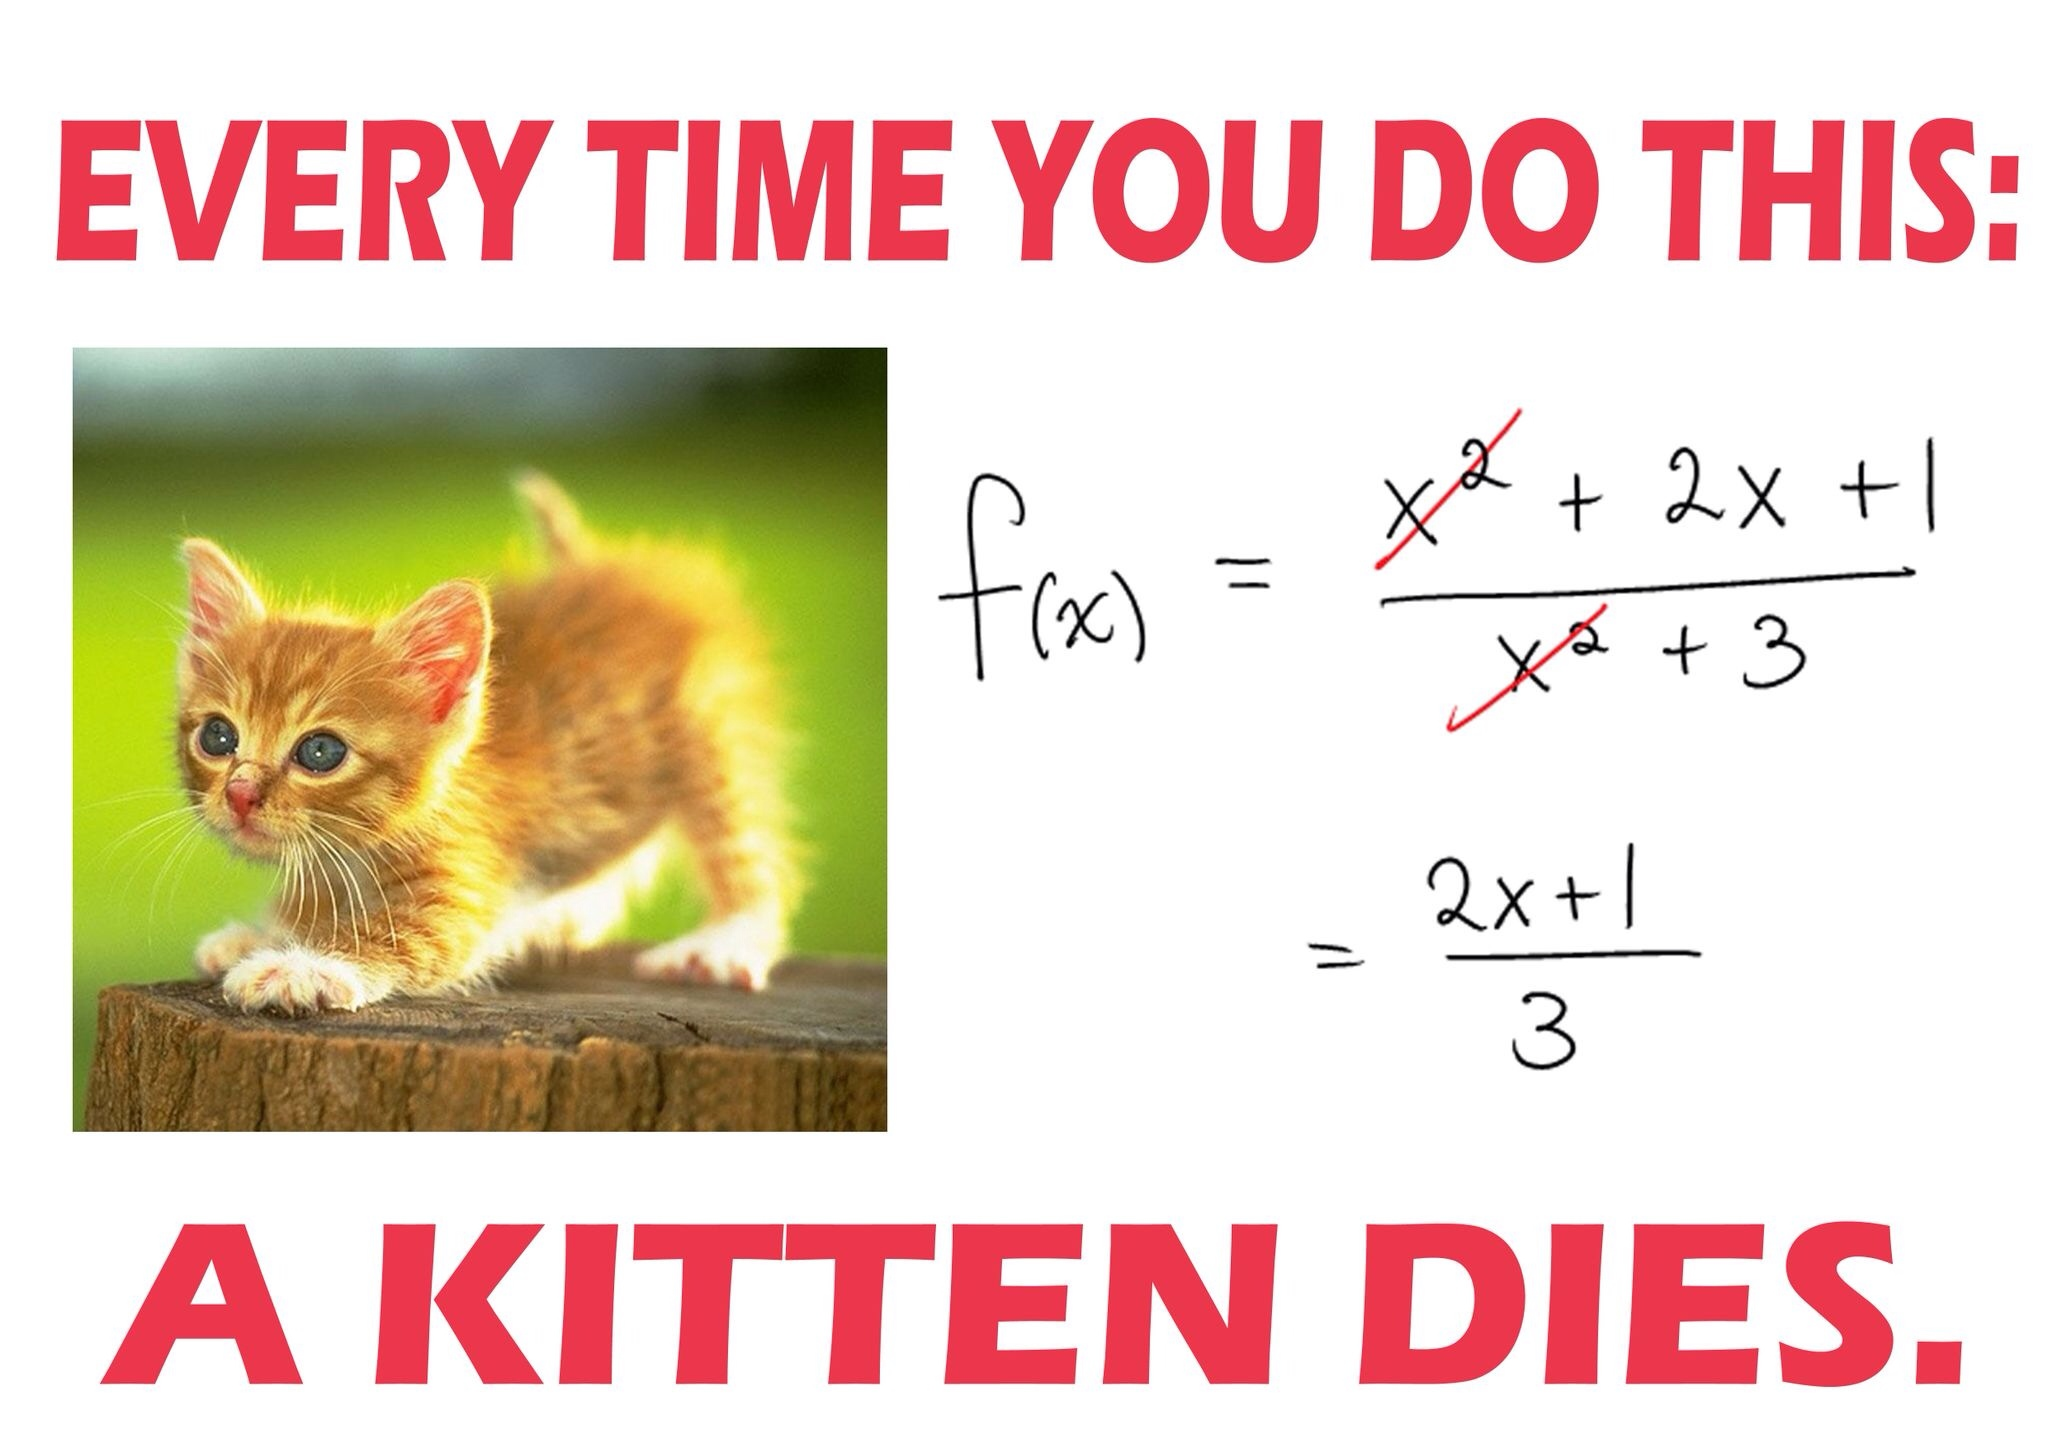
\includegraphics[width=6cm]{picture/obr.jpg}
\end{figure}
For example, considering a row of ten cells with spaces in the fifth and seventh cells and with clues of \textit{3} and \textit{2}:

\begin{itemize} 
 \item {the clue of \textit{3} would be forced to the left, because it could not fit anywhere else.}

\item {the empty gap on the sixth cell is too small to accommodate clues like \textit{2} or \textit{3} and may be filled with spaces.}

\item {finally, the clue of \textit{2} will spread through the ninth cell according to method \textit{Simple Boxes} above.} 
\end{itemize}



\section{Glue}
Sometimes, there is a box near the border that is not farther from the border than the length of the first clue. In this case, the first clue will spread through that box and will be forced outward from the border.
\begin{figure}
\centering
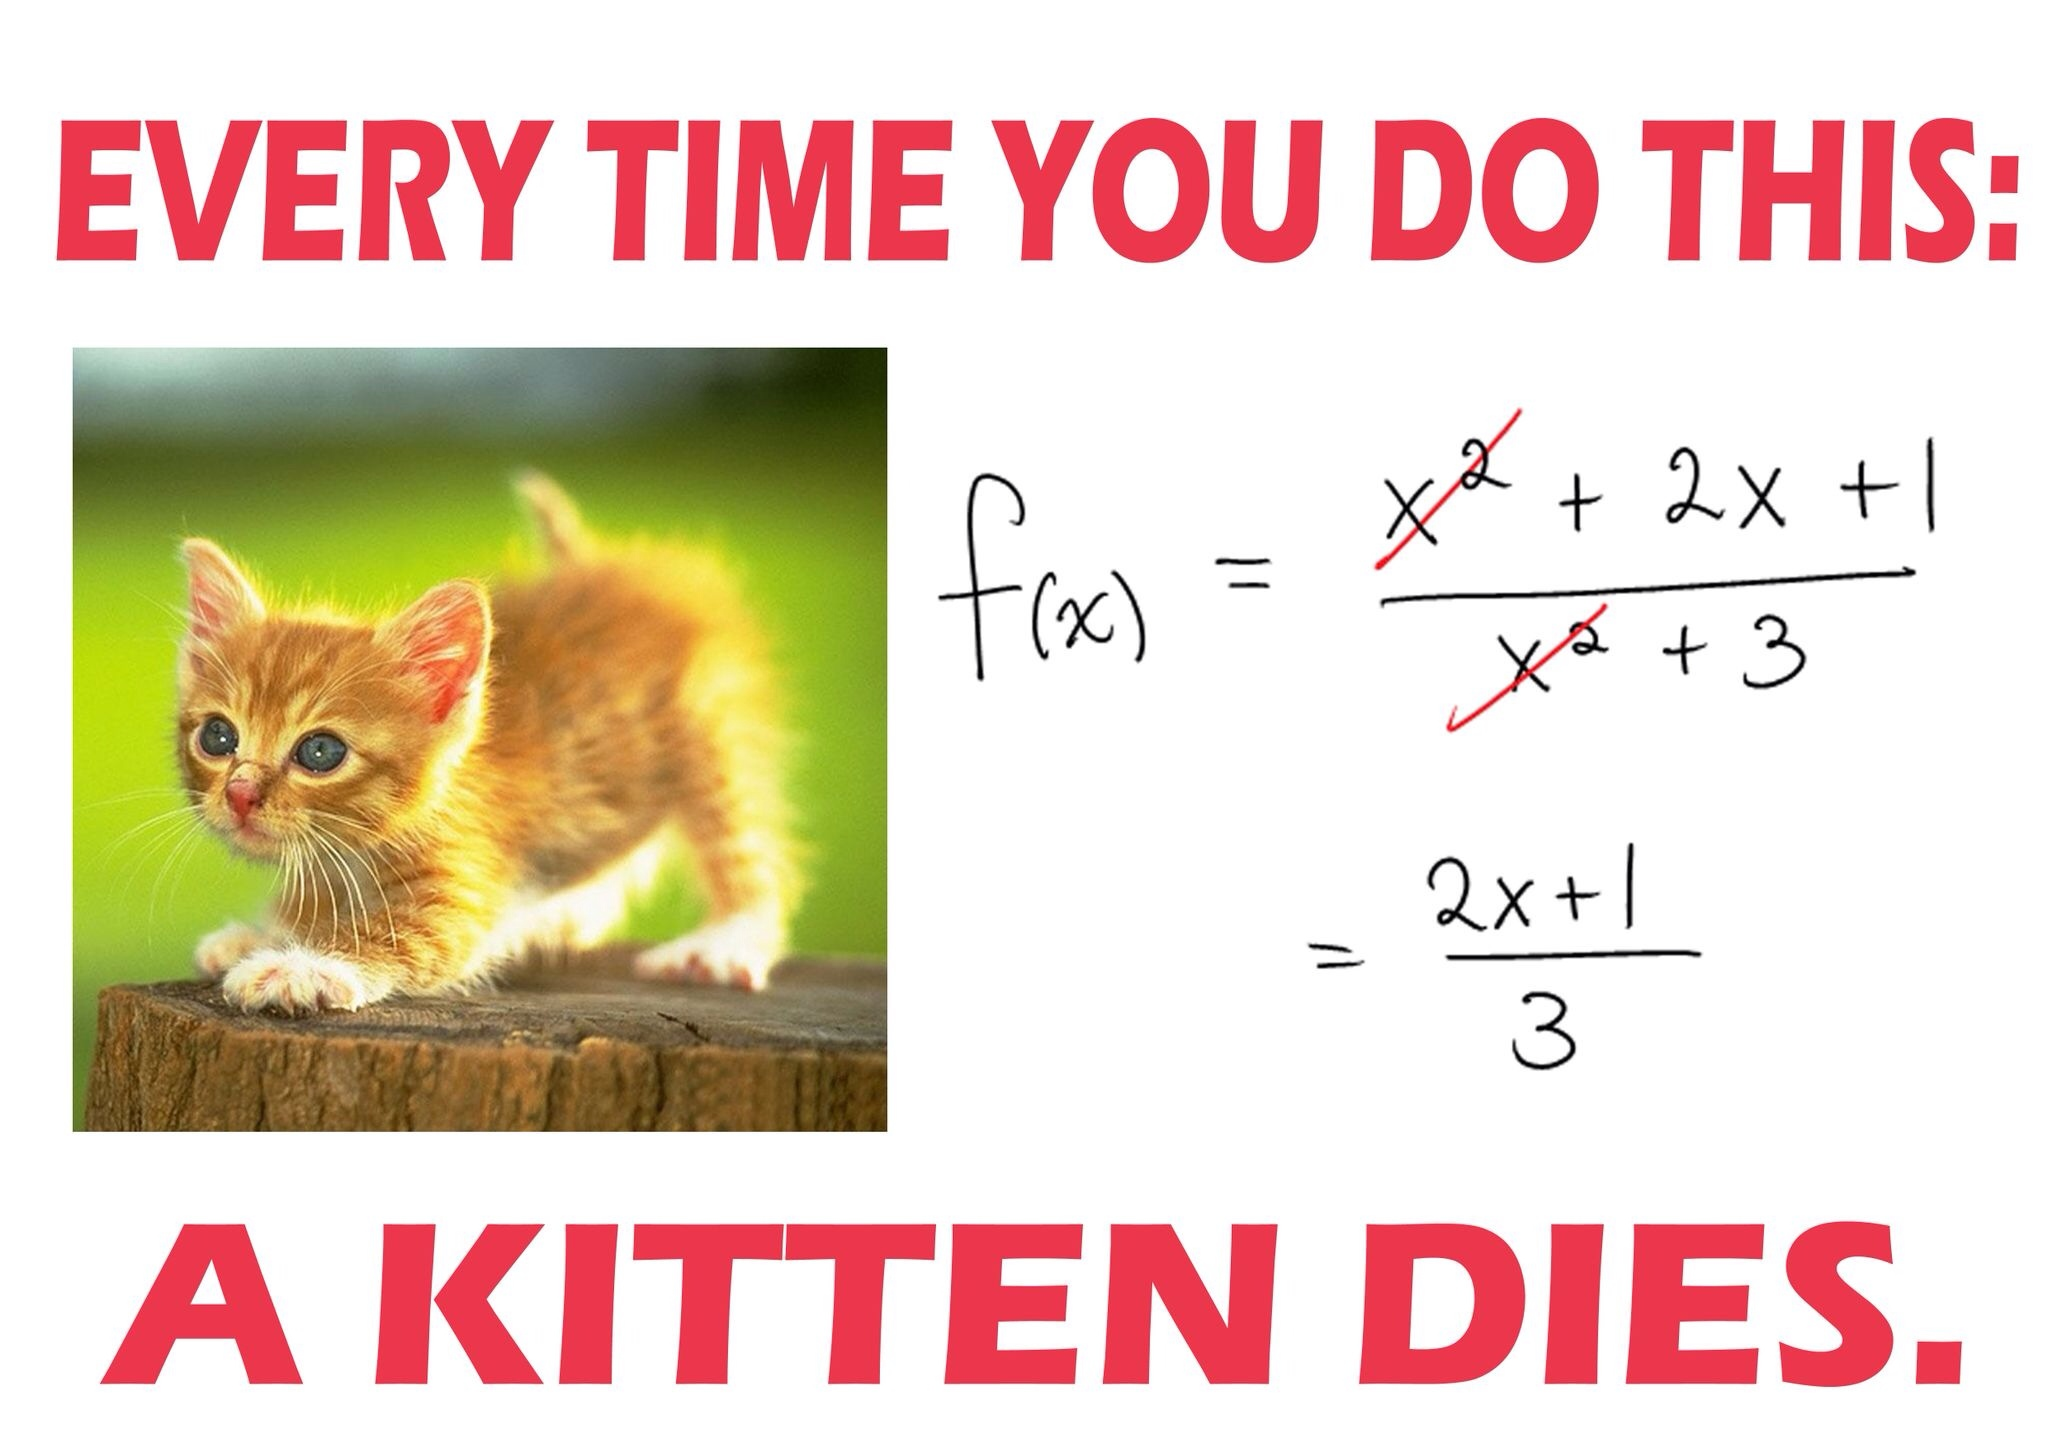
\includegraphics[width=6cm]{picture/obr.jpg}
\end{figure}
For example, considering a row of ten cells with a box in the third cell and with a clue of \textit{5}, the clue of \textit{5} will spread through the third cell and will continue to the fifth cell because of the border.

Note: This method may also work in the middle of a row, farther away from the borders.
\begin{figure}
\centering
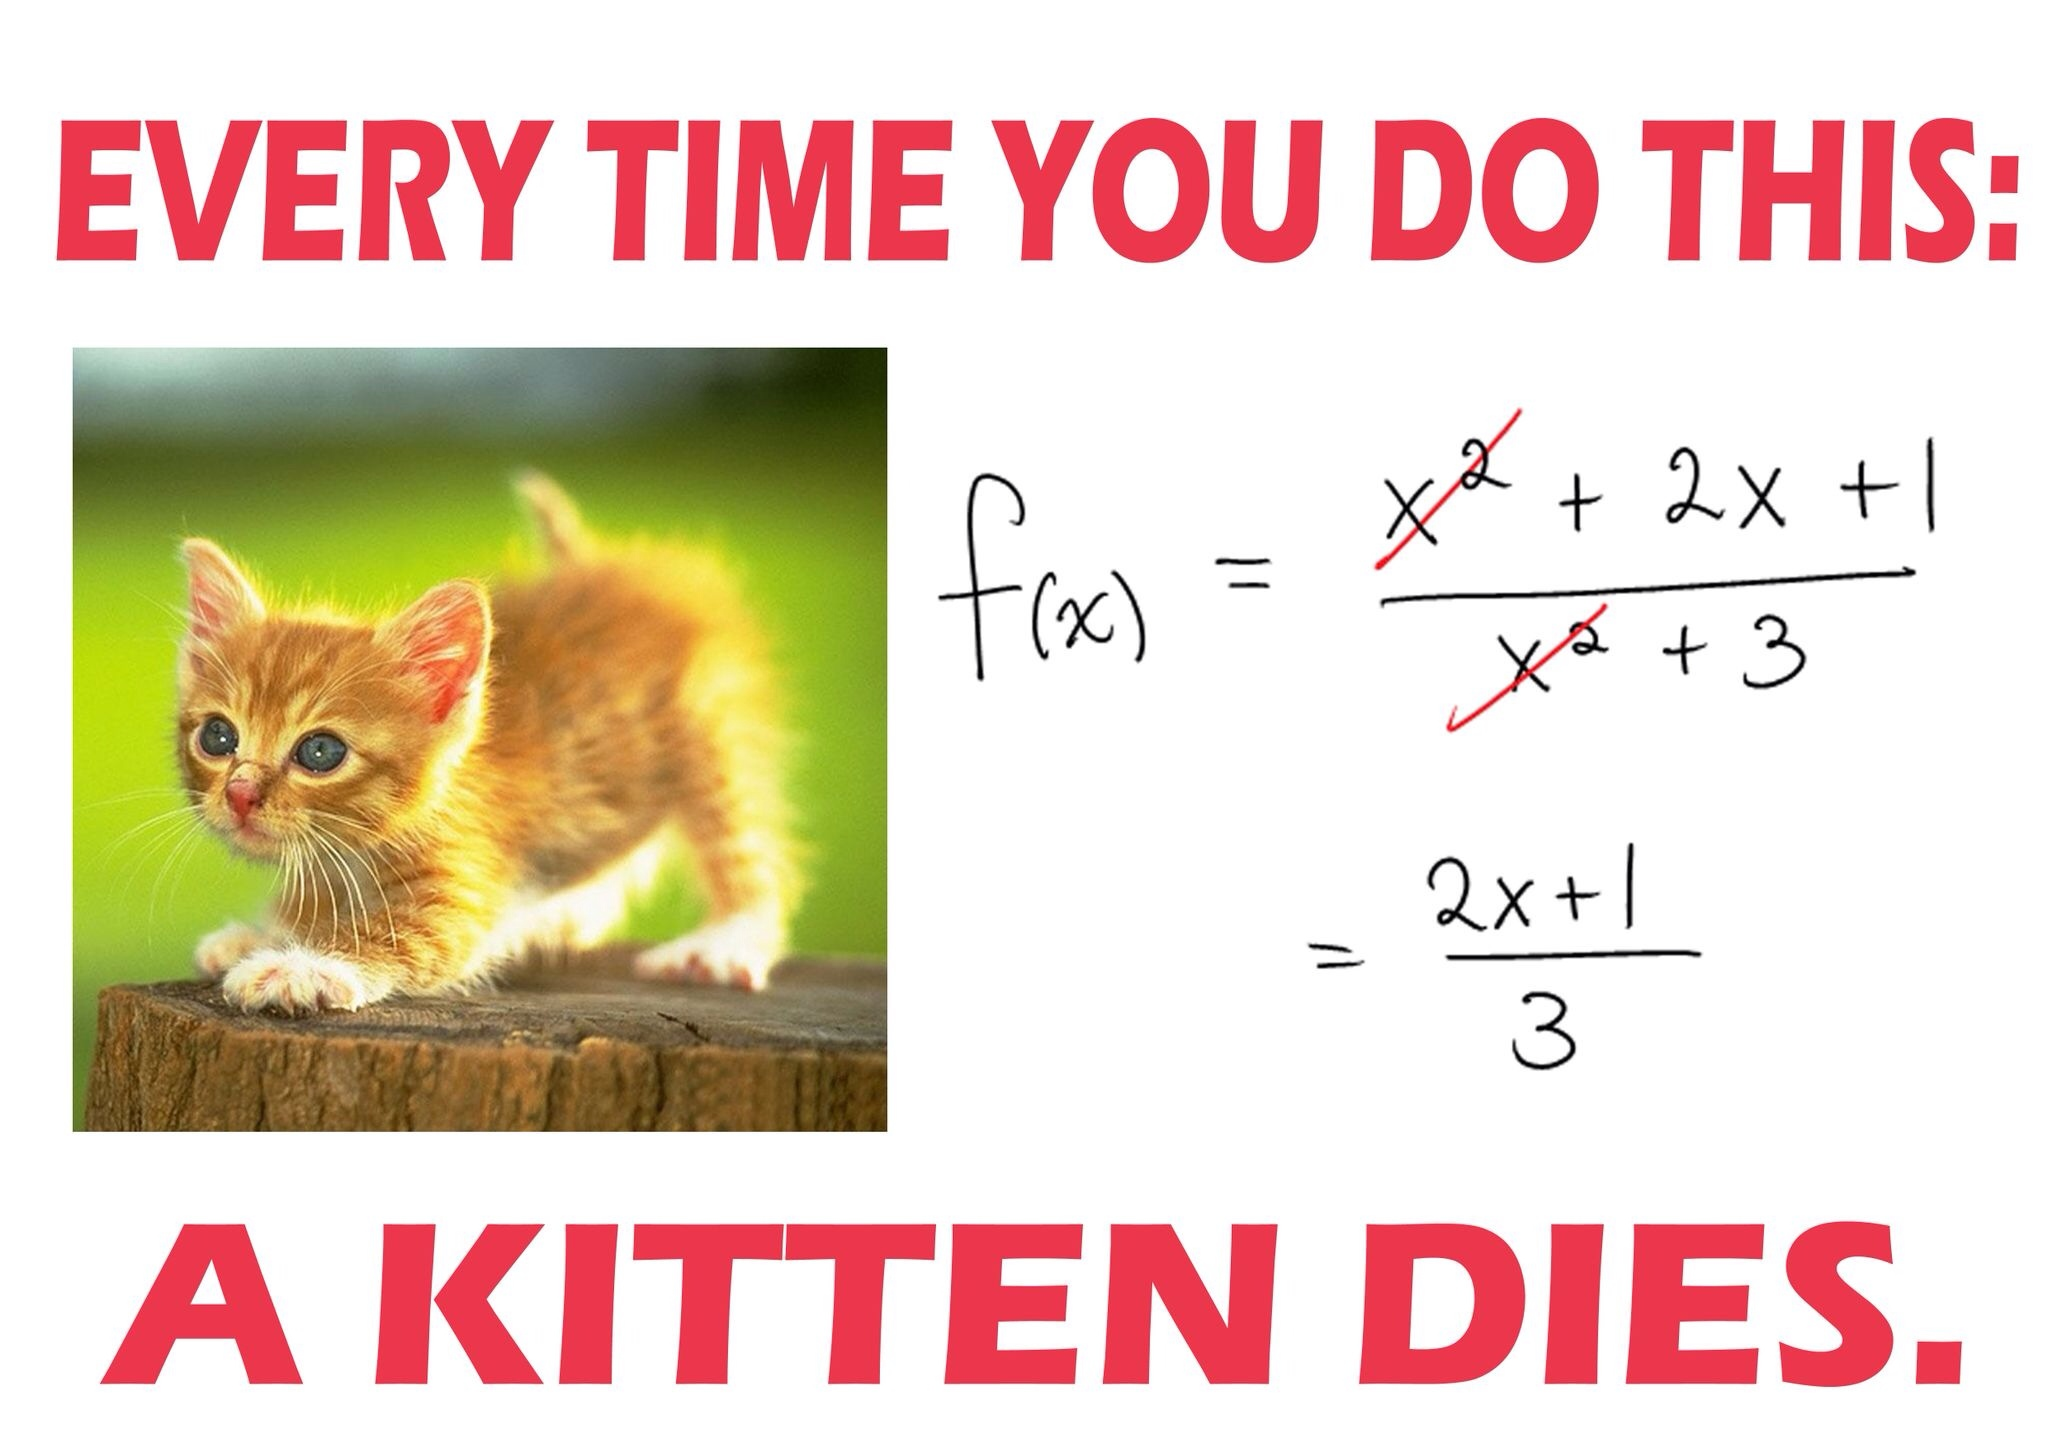
\includegraphics[width=6cm]{picture/obr.jpg}
\end{figure}

\begin{itemize} 
 \item {A space may act as a border, if the first clue is forced to the right of that space.}

\item {The \textit{first} clue may also be preceded by some other clues, if all the clues are already bound to the left of the forcing space.} 
\end{itemize}



\section{Joining and splitting}
Boxes closer to each other may be sometimes joined together into one block or split by a space into several blocks. When there are two blocks with an empty cell between, this cell will be:

\begin{itemize} 
 \item {A space if joining the two blocks by a box would produce a too large block}

\item {A box if splitting the two blocks by a space would produce a too small block that does not have enough free cells remaining} 
\end{itemize}


For example, considering a row of fifteen cells with boxes in the third, fourth, sixth, seventh, eleventh and thirteenth cell and with clues of \textit{5}, \textit{2} and \textit{2}:
\begin{figure}
\centering
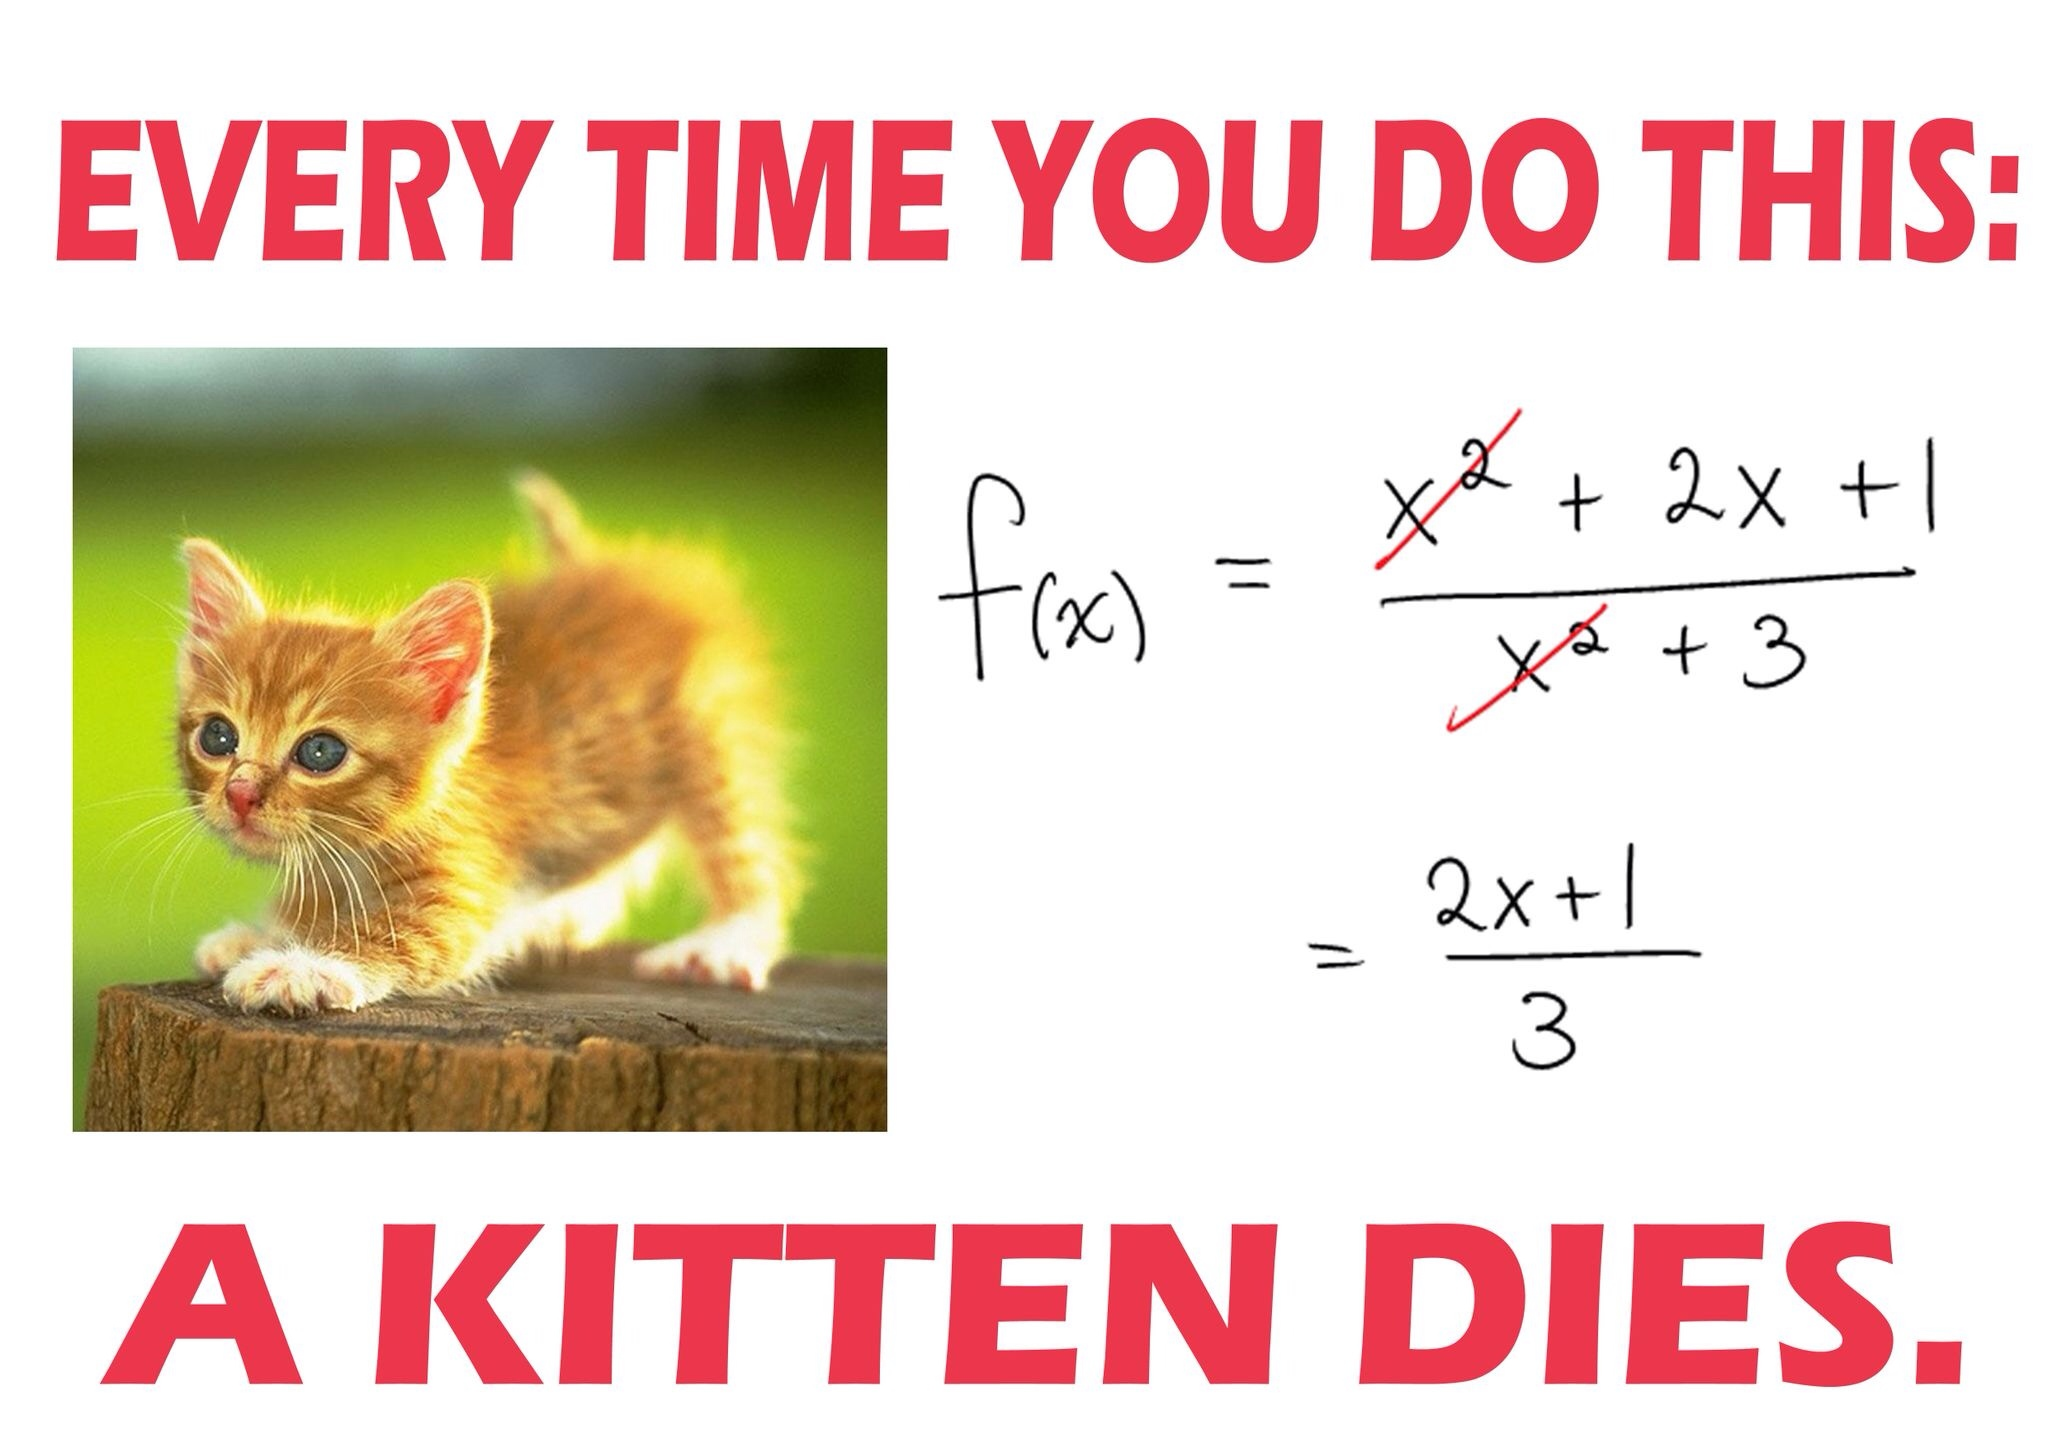
\includegraphics[width=6cm]{picture/obr.jpg}
\end{figure}

\begin{itemize} 
 \item {The clue of \textit{5} will join the first two blocks by a box into one large block, because a space would produce a block of only 4 boxes that is not enough there.}

\item {The clues of \textit{2} will split the last two blocks by a space, because a box would produce a block of 3 continuous boxes, which is not allowed there.} 
\end{itemize}

\textit{Note:} The illustration picture also shows how the clues of \textit{2} are further completed. This is, however, not part of the \textit{Joining and splitting} technique, but the \textit{Glue} technique described above.


\section{Punctuating}
To solve the puzzle, it is usually also very important to enclose each bound or completed block of boxes immediately by separating spaces as described in \textit{Simple spaces} method. Precise punctuating usually leads to more \textit{Forcing} and may be vital for finishing the puzzle. \textit{Note: The examples above did not do that only to remain simple.}


\section{Mercury}
\textit{Mercury} is a special case of \textit{Simple spaces} technique. Its name comes from the way \textit{mercury} pulls back from the sides of a container.
\begin{figure}
\centering
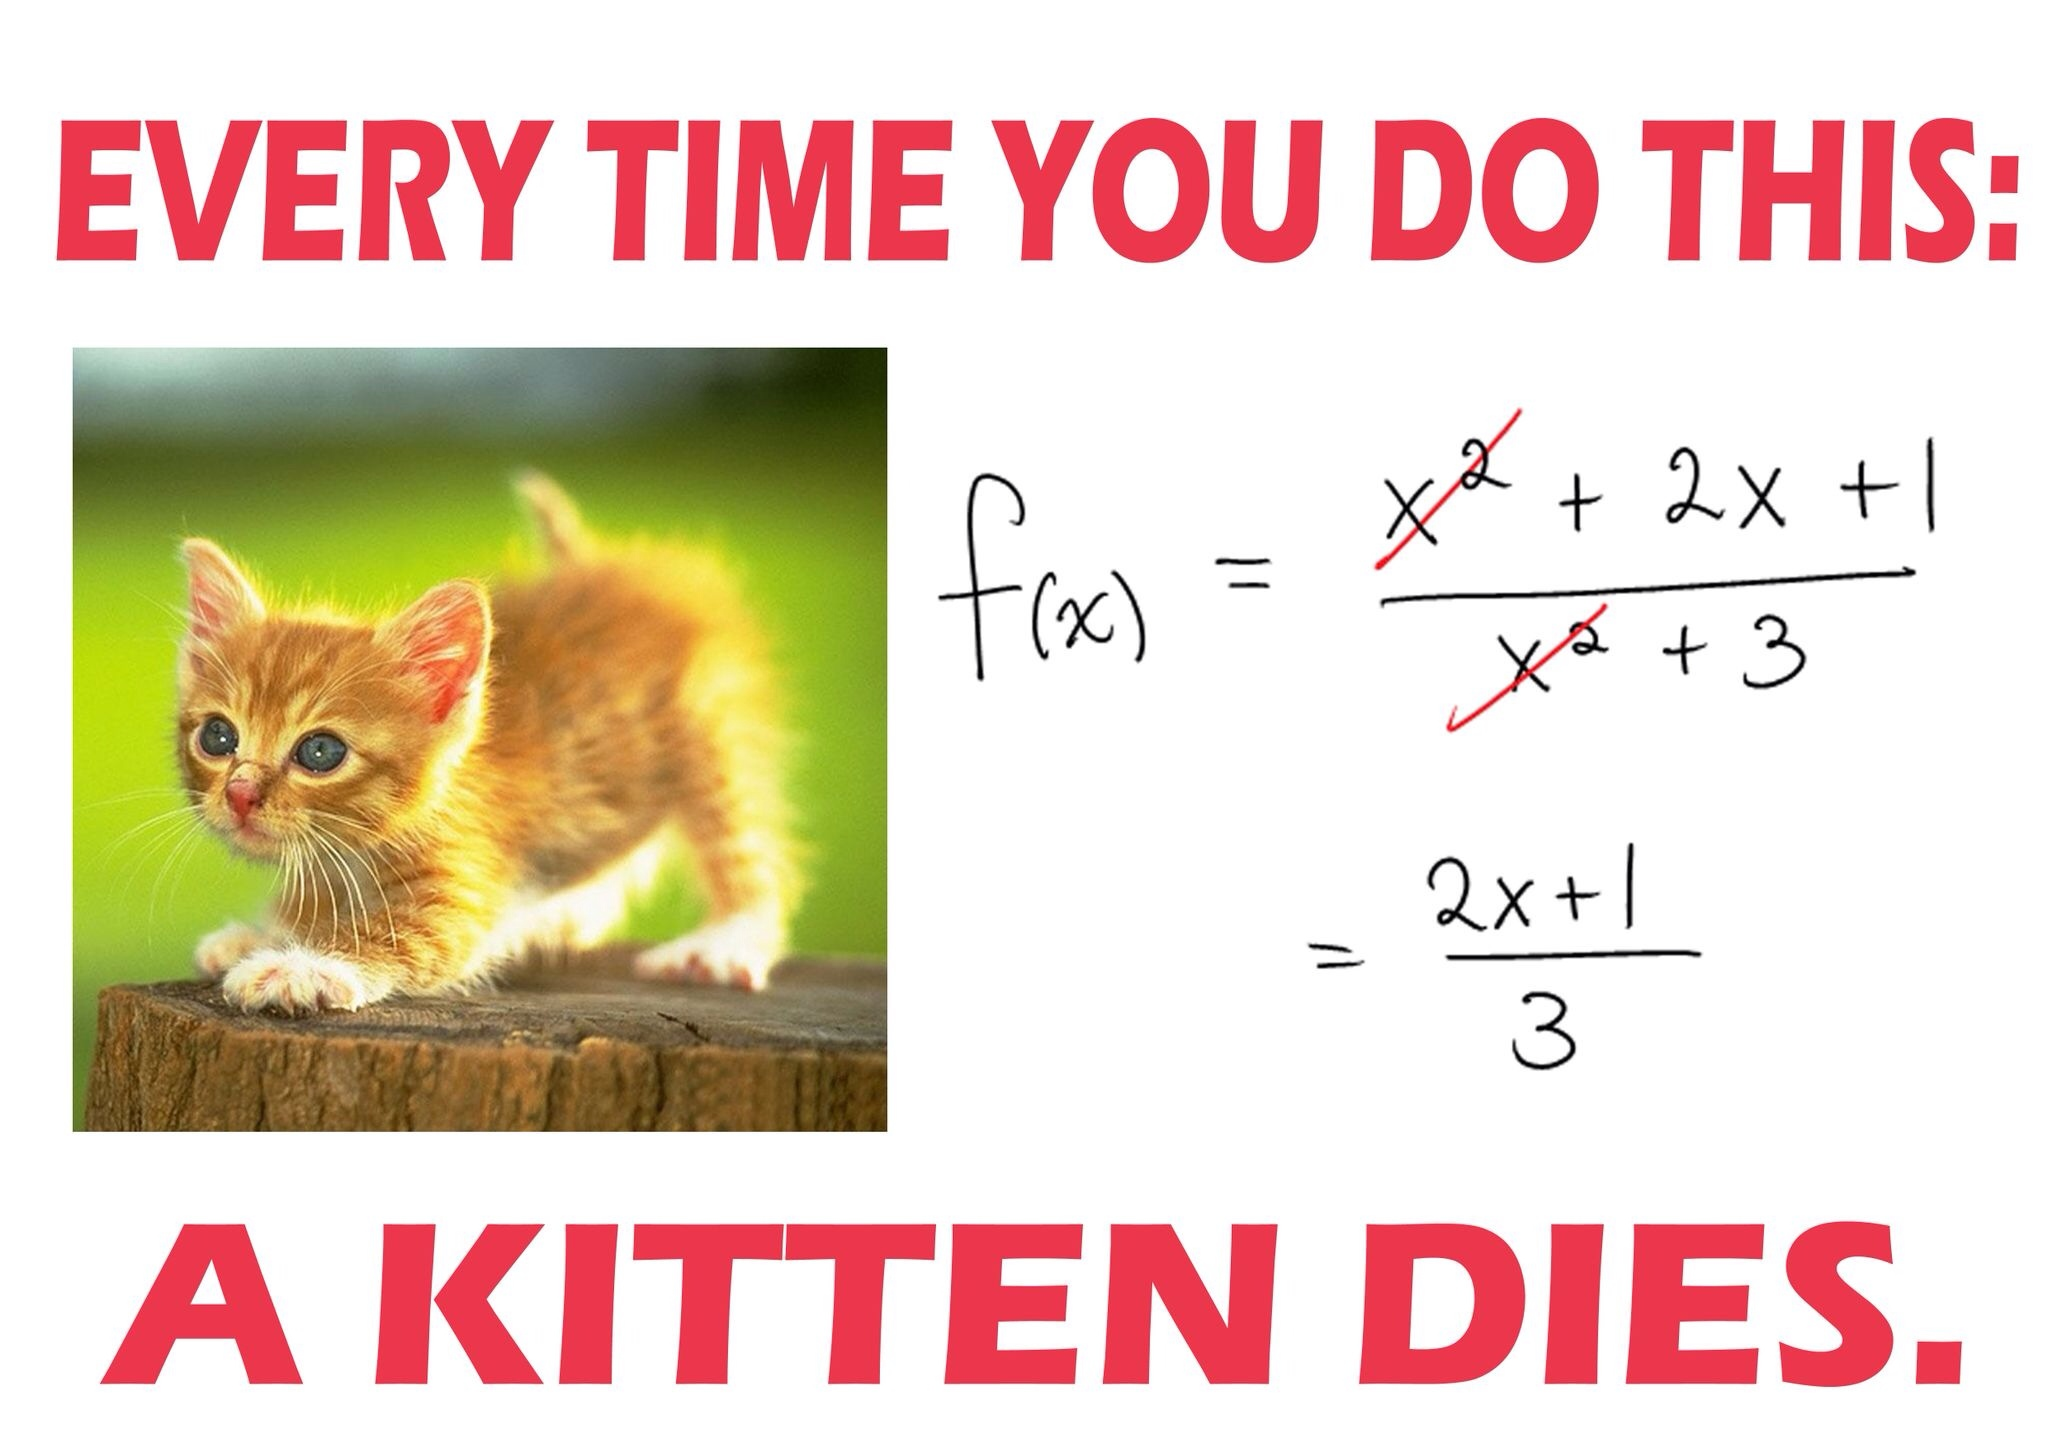
\includegraphics[width=6cm]{picture/obr.jpg}
\end{figure}
If there is a box in a row that is in the same distance from the border as the length of the first clue, the first cell will be a space. This is because the first clue would not fit to the left of the box. It will have to spread through that box, leaving the first cell behind. Furthermore, when the box is actually a block of more boxes to the right, there will be more spaces at the beginning of the row, determined by using this method several times.


\section{Contradictions}
Some more difficult puzzles may also require advanced reasoning. When all simple methods above are exhausted, searching for \textit{contradictions} may help. It is wise to use a pencil (or other color) for that to facilitate corrections. The procedure includes:

\begin{enumerate} 
 \item {Trying an empty cell to be a box (or then a space).}

\item {Using all available methods to solve as much as possible.}

\item {If an error is found, the tried cell will not be a box for sure. It will be a space (or a box, if space was tried).} 
\end{enumerate}


\begin{figure}
\centering
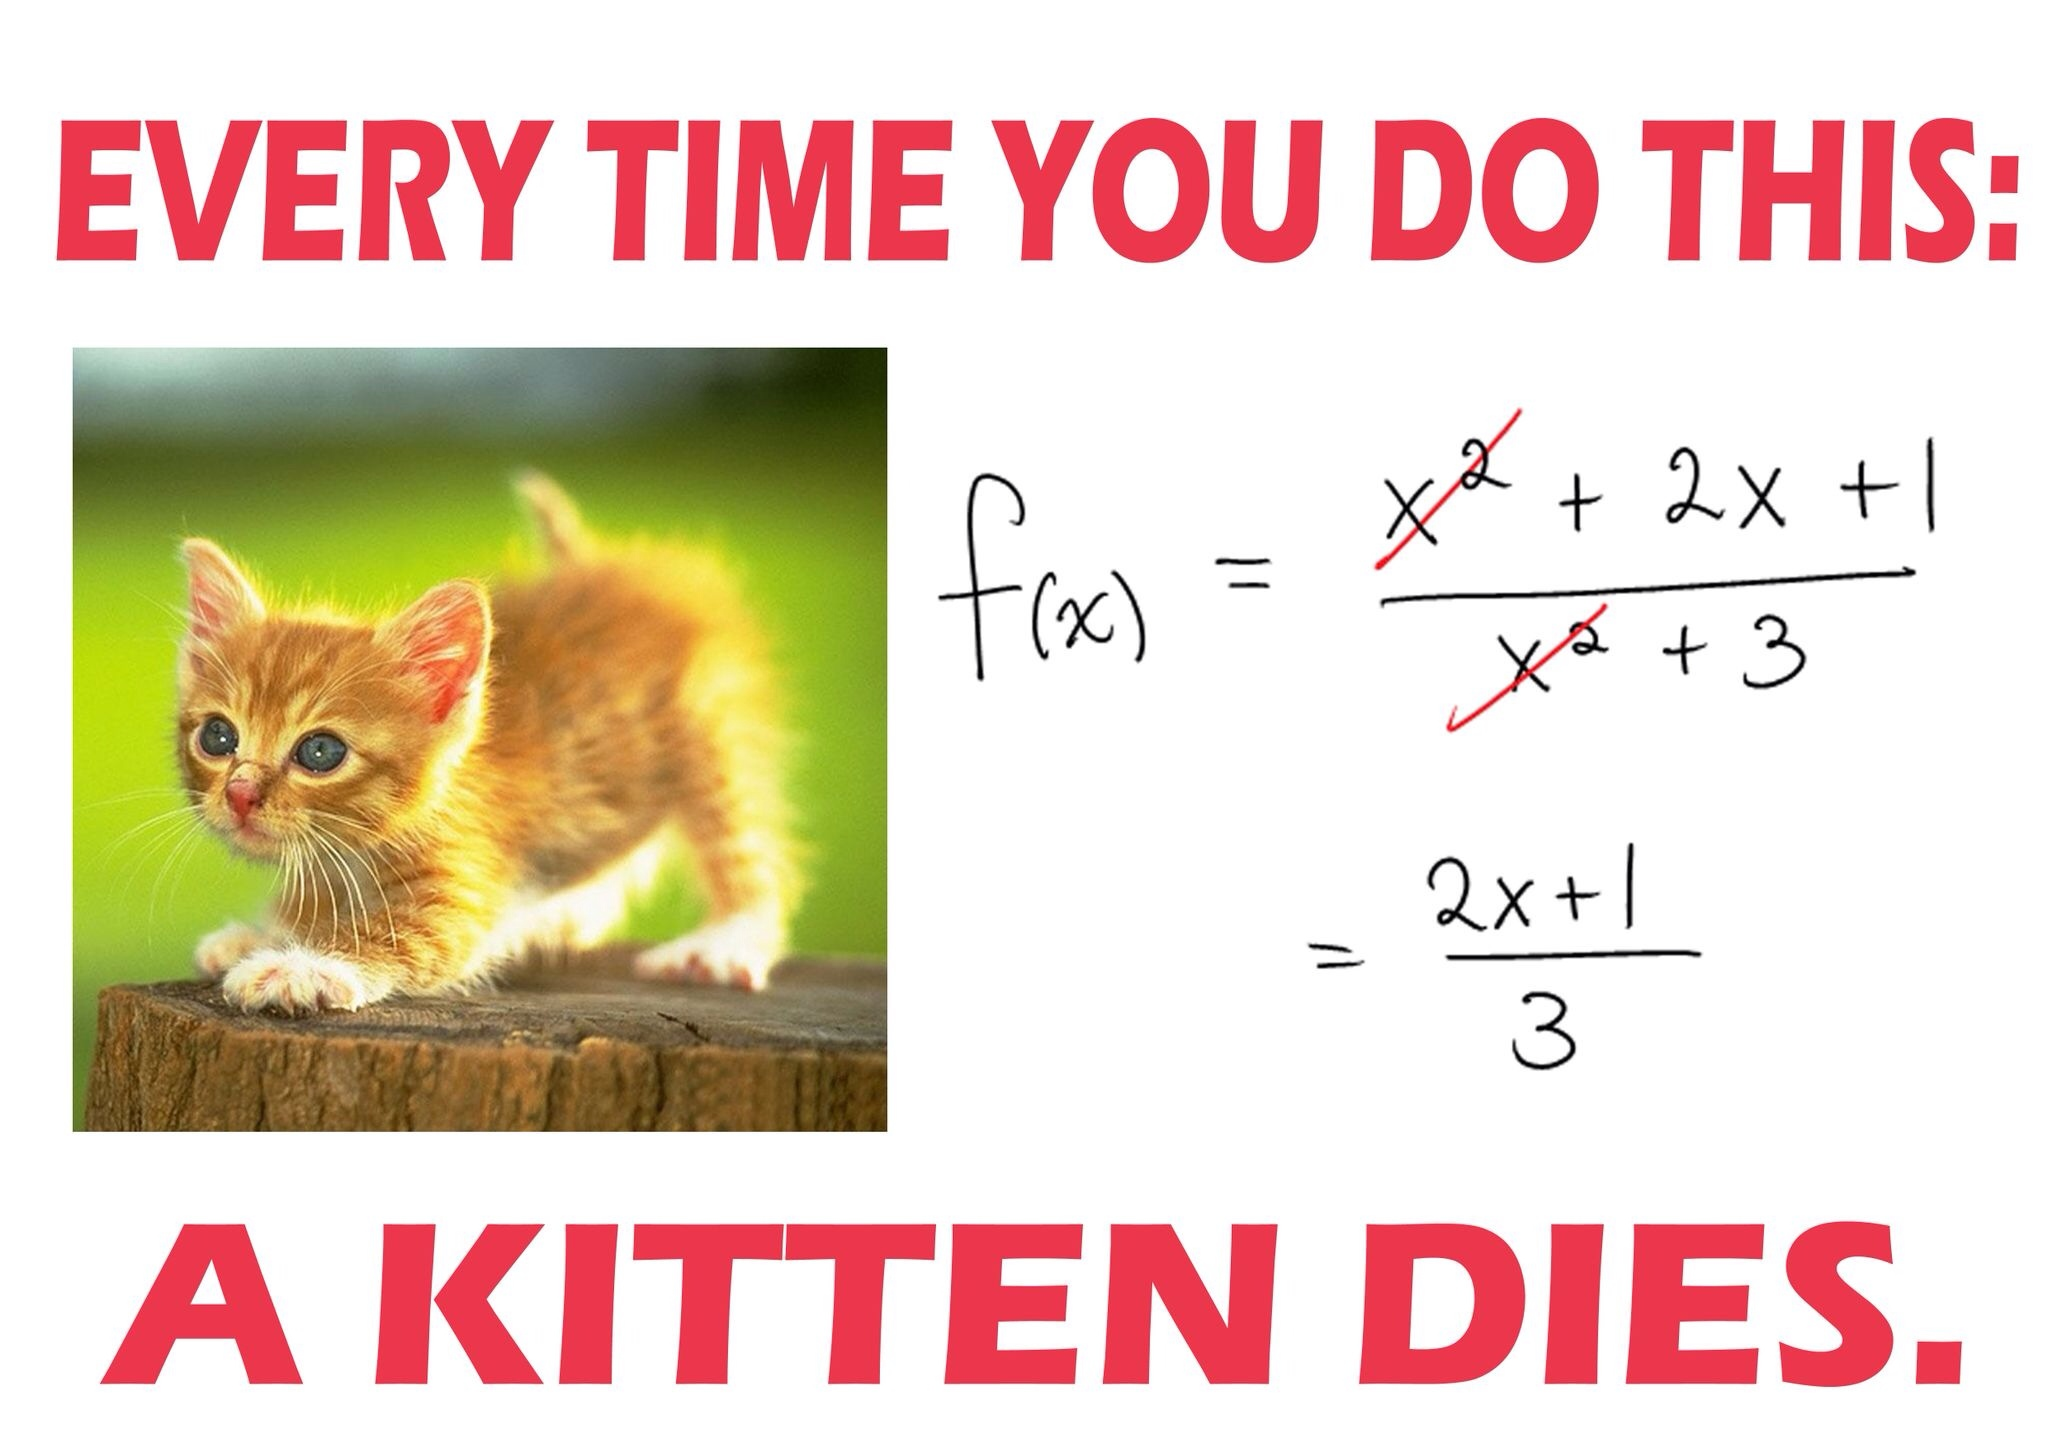
\includegraphics[width=6cm]{picture/obr.jpg}
\end{figure}

In this example a box is tried in the first row, which leads to a space at the beginning of that row. The space then \textit{forces} a box in the first column, which \textit{glues} to a block of three boxes in the fourth row. However, that is wrong because the third column does not allow any boxes there, which leads to a conclusion that the tried cell must not be a box, so it must be a space.

The problem of this method is that there is no quick way to tell which empty cell to try first. Usually only a few cells lead to any progress, and the other cells lead to dead ends. Most worthy cells to start with may be:

\begin{itemize} 
 \item {cells that have many non-empty neighbors;}

\item {cells that are close to the borders or close to the blocks of spaces;}

\item {cells that are within rows that consist of more non-empty cells.} 
\end{itemize}



\section{Deeper recursion}
Some puzzles may require to go deeper with searching for the contradictions. This is, however, not possible simply by a pen and pencil, because of the many possibilities that must be searched. This method is practical for a computer to use.


\section{Multiple rows}
In some cases, reasoning over a set of rows may also lead to the next step of the solution even without contradictions and deeper recursion. However, finding such sets is usually as difficult as finding contradictions.


\section{Multiple solutions}
There are puzzles that have several feasible solutions (one such is a picture of a simple \textit{chessboard}). In these puzzles, all solutions are \textit{correct} by the definition, but not all must give a reasonable picture.


\chapter{Nonograms in computing}
Solving nonogram puzzles is an \textit{NP-complete} problem.(TODO - referencia na literaturu)(TODO - referencia na literaturu)  This means that there is no \textit{polynomial time} \textit{algorithm} that solves all nonogram puzzles unless \textit{P = NP}.

However, certain classes of puzzles, such as those in which each row or column has only one block of cells and all cells are connected, may be solved in polynomial time by transforming the problem into an instance of \textit{2-satisfiability}.(TODO - referencia na literaturu)

Many nonograms can be solved efficiently, because the interrelated constraints on the two axes allow the search space to be \textit{bounded}, dramatically reducing the space that must be searched for a solution.


\chapter{Software solvers}

An extensive comparison and discussion of nonogram solving algorithms is found at the WebPBN site (Web Paint-By-Number).(TODO - referencia na literaturu)

Some other online and offline solvers include:


\begin{itemize} 
 \item {Teal nonogram puzzle and solver(TODO - referencia na literaturu)}

\item {Nonogram Solver(TODO - referencia na literaturu)}

\item {Griddlers solver with Animator(TODO - referencia na literaturu)}

\item {nonogram-solver (in Ruby)(TODO - referencia na literaturu)}

\item {nonogram-solver (in Python)(TODO - referencia na literaturu)}

\item {HTML5 Nonogram Solver (in browser)(TODO - referencia na literaturu)}

\item {Nonogram solver(TODO - referencia na literaturu) in C++ solving lines in quadratic time at most.(TODO - referencia na literaturu)}

\item {JavaScript Nonogram solver (TODO - referencia na literaturu)} 
\end{itemize}



\chapter{Video game versions}
\textit{Nintendo} have published several nonogram video games using the name . The \textit{Nintendo Game Boy} game \textit{\textit{Mario's Picross}} was initially released in Japan on March 14, 1995 to decent success. However, the game failed to become a hit in the U.S. market, despite a heavy advertising campaign by Nintendo. The game is of an escalating difficulty, with successive puzzle levels containing larger puzzles. Each puzzle has a limited amount of time to be cleared. Hints (line clears) may be requested at a time penalty, and mistakes made earn time penalties as well (the amount increasing for each mistake). \textit{Picross 2} was released later for Game Boy and \textit{\textit{Mario's Super Picross}} for the Super Famicom, neither of which were translated for the U.S. market (\textit{Mario's Super Picross} was, however, later released on the \textit{Wii} \textit{Virtual Console}'s PAL service on September 14, 2007, as part of its \textit{Hanabi Festival}). Both games introduced \textit{Wario's Picross} as well, featuring \textit{Mario's nemesis} in the role. These rounds vary by removing the hint function, and mistakes are not penalized - at the price that mistakes are not even revealed. These rounds can only be cleared when all correct boxes are marked, with no mistakes. The time limit was also removed. Nintendo also released eight \textit{Picross} volumes on the Japanese \textit{Nintendo Power} peripheral in Japan, each a new set of puzzles without the Mario characters.

Nintendo has released \textit{\textit{Picross DS}} for the \textit{Nintendo DS} portable system in 2007. It contains several stages of varying difficulty, from 5x5 grids to 25x20 grids. Normal mode tells players if they made an error (with a time penalty) and free mode does not. A hint is available before starting the puzzle in all modes; the game reveals a complete row and column at random. Additional puzzles were available through Nintendo Wi-Fi Connection; some of the original Mario Picross puzzles were available. However, the service was shut down on 20 May 2014. Nintendo made new releases available bi-weekly. \textit{Picross DS} was released in \textit{Europe} and \textit{Australia} on 11 May 2007 and in the \textit{United States} on July 30, 2007 and has been received well by critics, including Craig Harris,(TODO - referencia na literaturu) Matt Wadleigh(TODO - referencia na literaturu) and Dave McCarthy (TODO - referencia na literaturu) labelling the game "Addictive".(TODO - referencia na literaturu)(TODO - referencia na literaturu) A 3D version of the game, titled \textit{\textit{Picross 3D}}, was also released for the DS in Japan in 2009 and internationally in 2010. A sequel, \textit{\textit{Picross 3D: Round 2}}, was released for the \textit{Nintendo 3DS} in 2015.(TODO - referencia na literaturu) Another downloadable version of the game was released for Nintendo 3DS's Nintendo eShop, called \textit{Picross e}, \textit{Picross e2}, and \textit{Picross e3} released in 2013, with \textit{Picross e4} released in 2014. Nintendo has also released a \textit{Pokémon} spinoff on December 7, 2015 in the form of the \textit{freemium} game of \textit{\textit{Pokémon Picross}} for Nintendo 3DS. \textit{My Nintendo Picross \textit{The Legend of Zelda: Twilight Princess}} was released for Nintendo 3DS on March 31, 2016, exclusively as a premium reward for \textit{My Nintendo}.

Other companies have also released nonogram video games, such as Falcross(TODO - referencia na literaturu) on \textit{iOS}, and the Color Cross series of games by Little Worlds Studio on the Nintendo DS, \textit{Microsoft Windows}, and \textit{iOS}.


\chapter{Other picture logic puzzles}

\textbf{Pentomino paint-by-numbers} is a variant in which the twelve \textit{pentomino} shapes must be placed in the grid, without touching each other (even diagonally).

\textbf{Triddlers}(TODO - referencia na literaturu) are an offshoot that uses triangle shapes instead of squares.

\textbf{Paint by pairs} or \textbf{Link-a-Pix} consists of a grid, with numbers filling some squares; pairs of numbers must be located correctly and connected with a line filling a total of squares equal to that number.  There is only one unique way to link all the squares in a properly-constructed puzzle.  When completed, the squares that have lines are filled; the contrast with the blank squares reveals the picture. (As above, colored versions exist that involving matching numbers of the same color.)

\textbf{Fill-a-Pix} also uses a grid with numbers within. In this format, each number indicates how many of the squares immediately surrounding it, and itself, will be filled. A square marked "9," for example, will have all eight surrounding squares and itself filled. If it is marked "0" those squares are all blank.

\textbf{Maze-a-Pix} uses a maze in a standard grid.  When the single correct route from beginning to end is located, each 'square' of the solution is filled in (alternatively, all non-solution squares are filled in) to create the picture.

\textbf{Tile Paint} is another type of picture logic puzzle by Nikoli. It works like regular nonograms except that it only specifies the \textit{total} number of squares in each row or column that will be filled in and irregular sections within the grid have borders around them that indicate that, if one of the squares within it is filled in, all of them must be filled in.


\chapter{References}


